%-----------------------------------------------------------------------------
% Based on 15 February 2005 sigplanconf-template.tex by Paul C. Anagnostopoulos
%-----------------------------------------------------------------------------

\documentclass[12pt]{article}

\usepackage{bibspacing}
\usepackage{times}
\usepackage{amsmath}
\usepackage{psfig}
\usepackage{url}

\usepackage{simplemargins}
\setleftmargin{1.25in}
\setrightmargin{1.25in}
\settopmargin{1in}
\setbottommargin{1in}

\makeatletter
\font\elvbf  = cmbx10 scaled 1100
\def\section{\@startsection {section}{1}{\z@}
   {12pt plus 2pt minus 2pt}{8pt plus 2pt minus 2pt} {\large\bf}}
\def\subsection{\@startsection {subsection}{2}{\z@}
   {10pt plus 2pt minus 2pt}{4pt plus 1pt minus 1pt} {\bf}}
\makeatother

\newcommand{\eightpoint}{\fontsize{8pt}{10pt}\selectfont}
\newcommand{\ninepoint}{\fontsize{9pt}{11pt}\selectfont}
\newcommand{\tenpoint}{\fontsize{10pt}{12pt}\selectfont}
\newcommand{\elevenpoint}{\fontsize{11pt}{13pt}\selectfont}
\newcommand{\thirteenpoint}{\fontsize{13pt}{14pt}\selectfont}
\newcommand{\fourteenpoint}{\fontsize{14pt}{16pt}\selectfont}

\begin{document}

%\conferenceinfo{POPL '06}{January 2007, Nice, France.} 
%\copyrightyear{2007}
%\copyrightdata{[to be supplied]}

%\titlebanner{banner above paper title}        % These are ignored unless
%\preprintfooter{short description of paper}   % 'preprint' option specified.

\title{\vspace{-40pt} \Large Direct Manipulation of LZ77-Compressed Data}
%\title{\vspace{-40pt} \Large Compressed-Domain Techniques for Lossless Formats}

%\title{\Large Compressed-Domain Techniques for Lempel-Ziv Formats}
%\title{\Large Compressed-Domain Transformation of Lossless Image and Video Encodings}

%\authorinfo{}

\author{\vspace{-24pt} ~ \\ \thirteenpoint William Thies, Steven Hall, and Saman Amarasinghe \\
        \thirteenpoint MIT Computer Science and Artificial Intelligence Laboratory \\ \vspace{-48pt}}

\date{}
%	    Massachusetts Institute of Technology}
%           {\{thies,saman\}@mit.edu}

\maketitle

\begin{abstract}
Due to the high data rates involved in audio, video, and signal
processing applications, it is imperative to compress the data to
decrease the amount of storage used.  Unfortunately, this implies that
any program operating on the data needs to be wrapped by a
decompression and re-compression stage.  Re-compression can incur
significant computational overhead, while decompression swamps the
application with the original volume of data.

In this paper, we present a program transformation that greatly
accelerates the processing of compressible data.  Given a program that
operates on uncompressed data, we output an equivalent program that
operates directly on the compressed format.  Our transformation
applies to stream programs, a restricted but useful class of
applications with regular communication and computation patterns.  Our
formulation is based on LZ77, a lossless compression algorithm
utilized by ZIP, and immediately applies to simpler formats such as
Apple Animation, Microsoft RLE, and Targa.

We implemented a simple subset of our techniques in the StreamIt
compiler, which emits executable plugins for two popular video editing
tools: MEncoder and Blender.  For common operations such as color
adjustment and video compositing, computing directly on compressed
data offers a speedup roughly proportional to the overall compression
ratio.  For our benchmark suite of 12 videos in Apple Animation
format, speedups range from 1.1x to 471x, with a median of 15x.

\end{abstract}

%% \category{CR-number}{subcategory}{third-level}
%%
%% \terms
%% term1, term2
%%
%% \keywords
%% keyword1, keyword2

\section{Introduction}


Stream computing represents an increasingly important class of
applications. In streaming codes, there is an abundance of parallelism that
is easier to extract compared to traditional desktop workloads (e.g.,
pointer-based computing). As a result, the extraction of parallelism
in streaming codes does not require heroic efforts, and thus,
processors can deliver higher performance with significantly lower
power costs. This is especially important since
leading microprocessor companies have realized that modern general
purpose architectures are near their  performance limits for  the
amount of power they consume. Thus, the future will place a greater
emphasis on exploiting the properties of streaming workloads in
conventional von~Neumann architectures.

Streaming is a model of computation that uses sequences of data
and computation kernels to expose concurrency and locality for
efficiency~\cite{wss}. In general purpose processors, improving locality 
translates to an effective management of the memory hierarchy at all
levels, including the register file. In this paper, we present a
methodology for compiling streaming codes to general purpose,
cache-based architectures. We first introduce a simple model for
reasoning effectively about the caching behavior of streaming
workloads. This model serves as a foundation for several {\it cache-aware
optimizations} that are geared toward the concomitant increase of instruction
and data {\it temporal locality}. These
optimization lead to significantly better utilization of the memory
system, and as such, they deliver performance gains ranging from 11
to 99\% for our streaming benchmark suite.

The context for our work is StreamIt, an architecture-independent
language that is engineered for streaming
applications~\cite{streamitcc}. It adopts the 
Cyclo-Static Dataflow~\cite{BELP96} model of computation which is a
generalization of Synchronous Dataflow~\cite{LM87-i} (SDF).  
SDF is a popular  model that  is well suited for
streaming codes. In SDF, computation is represented as a graph
consisting of {\it  actors} connected by communication channels; the
actors consume  and produce a constant number  of items from their
input and output  channels every time they execute. SDF is appealing
because it is amenable to static scheduling and optimization. 

From a general purpose architecture's point of view, actors represent
computation kernels, and the communication between actors represents
data buffers that must be streamed to and from the processor. Thus
the size of an actor and the
order of actor executions are critical properties that
impact the performance of the instruction cache. For example, the
compiler must make sure the actor's code size is not
greater than the instruction cache. Furthermore, we must {\it scale}
the execution of the actor so that it runs several times before we move
on to some other actor in the stream 
graph. This serves to $(i)$ amortize the cost of fetching the actor's
instructions into the cache from memory (an expensive operation), $(ii)$
improve the instruction temporal locality, and $(iii)$ improve overall
performance. However, as our cache model will show, we 
cannot arbitrarily scale the execution frequency of an actor. This
is because actors produce data that must be buffered, and therefore,
we must also consider the amount of data an actor produces and
consumes if we are to adequately manage the data cache. This paper is unique
in that it is the first to present a unified optimization methodology
that simultaneously considers instruction and data locality for
mapping streaming computation to cache-based architectures.

In terms of improving the data cache behavior, the compiler schedules
actor firing such that the producer-consumer locality is
preserved. Furthermore,  the compiler may {\it fuse}
together two or more actors to form a coarser grained kernel.
The fusion allows for better register allocation as we can
destroy the arrays used to buffer data between the actors and replace
the corresponding array references with scalars.  It also allows for
various competing implementations for managing the buffers between the
fused actors.  This paper evaluates several implementation
alternatives (for buffer management) and evaluates their performance.

The methodology for fusing actors leverages a distinguishing StreamIt
characteristic, namely, the hierarchical organization of
the stream graph. Furthermore, the algorithm for fusing actors applies
for the various topologies allowed by StreamIt.
It also considers another distinguishing characteristics of StreamIt,
namely the {\tt peek} operation whereby an actor may inspect data
items in its input buffer without consuming them until some future
execution. While peeking is a powerful language feature, it does pose
some challenges to the compiler and the cache optimizations. Peeking
also impacts the choice for the best buffer management strategy, as our
study will show.

%% the comment about p3 and itanium not being embedded architectures
%% is out of the blue! need a better transition.
Cache-aware fusion alone delivers significant performance gains, although our
evaluation shows that fusion with scaling leads to the best
performance on a general purpose, cache-based architecture. For our
experiments, we use two different processors: a superscalar out-of-order
processor, and an in-order VLIW processor. The former is a Pentium~3
whereas the latter is an Itanium~2. While these architectures are not
particularly suited for an embedded system, they do exhibit some
properties that are worthy of investigation. Furthermore, that we can
demonstrate measurable performance gains on real systems is far more
convincing than using a simulation-based environment. We chose the
Pentium~3 processor because it has very few registers in its
instruction set architecture. The Itanium by contrast has a much 
larger and richer repertoire of registers. The two architectures serve
to validate our cache-aware optimizations, in that we expect an
architecture with more register to benefit more from optimization such
as scalar replacement. On average, fusion leads to a 47\% improvement
on the Pentium~3, and 50\% on the Itanium~2.

The two architectures also differ in terms of their memory system
organization. The Itanium is an in-order VLIW processor and does not
tolerate a memory stall as well as its out-of-order
counterpart. Therefore we expect different gains from the scaling
optimization which amortize the long access latencies for instruction
and data caches. On average, scaling leads to a 21\% improvement on
the Itanium~2, and 17\% on the Pentium~3.

While both scaling and fusion lead to modest performance gains, we
must combine the two to deliver the best possible performance. When we
do so, we can further improve the performance of our benchmarks by
53\% on average for the Pentium~3, and 55\% for the Itanium~2.

\subsection{Summary of Contributions}

This paper makes the following contributions:
\begin{itemize}

\item A cache model for stream computing that provides a quantitative
estimate of the caching performance for any sequence of actor
executions.

\item A cache-aware scheduling heuristic that judiciously increases
the multiplicity of actors, improving instruction and data locality
while not exceeding the data cache.

\item A cache-aware partitioning policy that judiciously fuses
adjacent actors into a single component, enabling local optimizations
while not exceeding the instruction cache.

\item An optimized buffer management policy, termed ``copy-shift with
execution scaling'', which out-performs a traditional rotating buffer
in a detailed micro-benchmark analysis.

\item A fully automatic implementation of the above techniques in the
StreamIt compiler.

\item An experimental evaluation across 11 streaming benchmarks,
demonstrating performance improvements of up to 99\%.
\end{itemize}

\subsection{Paper Roadmap}

The remainder of the paper is organized as follows. Section~\ref{sec:streamit}
describes StreamIt and introduces our motivating example.
Section~\ref{sec:cache-model} introduces our cache model for 
reasoning about the performance of a streaming
computation. Section~\ref{sec:cache-opt} describes our cache-aware
optimizations, and Section~\ref{sec:buffer} describes the 
optimization enabled by fusion. Section~\ref{sec:evaluation} describes
our evaluation methodology and present our experimental
analysis. Sections~\ref{sec:related-work}~and~\ref{sec:conclusion}
discuss related work and concludes the paper.

% RULE APPEARANCE:
\newcommand{\x}{\hspace{1.3pt}} % arithmetic multiplication symbol
\newcommand{\concat}[0]{\bullet}               % list concatenation symbol
\newcommand{\name}[1]{~~\hfill\framebox{#1}}   % for labeling rules

% RULE SPACING:
\newcommand{\skiptop}[0]{\vspace{-13pt}\\}   % for single line on top
\newcommand{\skiptopa}[0]{\vspace{-1pt}\\}   % for first line of two-line top part
\newcommand{\skiptopb}[0]{\vspace{-3pt}\\}   % for second line of two-line top part
\newcommand{\skipbot}[0]{\vspace{-3pt}\\}    % for single line on botto

% HELPER FOR REPEATS:
\newcommand{\tup}[2]{\langle#1, #2\rangle}

% OUR LABEL FOR THE ``POS'' VARIABLE
\newcommand{\pos}[0]{\mbox{\it pos}}

% MY TAB STOP FOR THE PSEUDOCODE
\newcommand{\tab}[0]{\mbox{~~~~}}

%%%%%%%%%%%%%%%%%%%%%%%%%%%%%%%%%%%%%%%%%%%%%%%%%%%%%%%%%%%%%%%%%%%%%%%%%%

\enlargethispage{0.5pt}
\section{Program Representation}

Our transformation relies on the cyclo-static dataflow representation
for input programs and the LZ77 representation of compressed data.
These are described in the next two sections.

\subsection{Cyclo-Static Dataflow}

In the cyclo-static dataflow model, a program is represented by a set
of independent {\it actors} that communicate using FIFO data
channels~\cite{bilsen95-cyclostatic,LM87-i}.  Each actor has an
independent program counter and address space; all communication is
done using the data channels.  Actors have one or more atomic
execution steps that execute in a fixed pattern throughout the
lifetime of the program.  A key restriction of the cyclo-static
dataflow model is that, for each execution of a given actor, the
number of items produced and consumed on the data channels is known at
compile time.  This enables the compiler to perform static scheduling
of the actors and to guarantee deadlock freedom~\cite{bilsen95-cyclostatic,LM87-i}.

Cyclo-static dataflow is a natural fit for many multimedia and signal
processing kernels, as such programs often have a regular structure
with known communication patterns.  As a programmer, one can use a
high-level language such as StreamIt~\cite{streamitcc} to express a
cyclo-static dataflow program.  An example StreamIt program appears in
Figure~\ref{fig:streamit}.  It reads lines of an RGB image from a
file, shrinks the image by a factor of two, inverts the color of each
pixel, then writes the data to a file.  There are three kinds of
actors in StreamIt programs, and our analysis handles each one
separately:
\begin{itemize}

\item {\bf Filters} have a single input stream and a single output
  stream, and perform general-purpose computation.  Filters perform
  the same function on every execution (there is no cyclic pattern of
  computations).  For example, in the {\tt InvertColor} filter, the
  {\tt work} function specifies the atomic execution step; it declares
  that on each execution, it pops (inputs) 1 item from the input tape
  and pushes (outputs) 1 item to the output tape\footnote{Though
    StreamIt also allows filters to peek at the input stream (i.e., to
    perform a sliding window computation) and to maintain mutable
    state across executions, these features are uncommon in other
    stream languages and we do not support them in the current work.}.

\item {\bf Splitters} have a single input stream and multiple output
  streams, and perform pre-defined computations.  There are two types
  of splitters: {\it duplicate} splitters, which replicate their
  inputs to all of the target streams, and {\it roundrobin} splitters,
  which distribute the input items across the streams.  Roundrobin
  splitters are parameterized: roundrobin$(n_1, n_2)$ indicates that
  the first $n_1$ items are sent to the first output, and the next
  $n_2$ items are sent to the second output.  Splitters execute in a
  fine-grained, cyclo-static fashion: regardless of the parameters,
  each execution step passes only a single item from the input stream
  to an output stream.  In Figure~\ref{fig:streamit}, the splitter
  sends {\tt WIDTH} pixels in each direction, distributing the lines
  of the image across alternate streams.

\begin{figure}[t]
\psfig{figure=streamit-figure.eps,width=3.408in}
\caption{Example StreamIt program.
\protect\label{fig:streamit}}
\end{figure}

\item {\bf Joiners} have multiple input streams and a single output
  stream, and perform pre-defined computations.  The only type of
  joiner is roundrobin, which acts analogously to a roundrobin
  splitter.  In Figure~\ref{fig:streamit}, the joiner reads one pixel
  at a time from each input stream, serving to interleave the pixels
  from neighboring lines.  Once the pixels are interleaved, each group
  of 4 pixels is averaged together in order to decrease the picture
  width by two.

\end{itemize}

\subsection{LZ77 Compression}

LZ77 is a lossless, dictionary-based compression algorithm.  Named
after its creators Lempel and Ziv, who published the algorithm in
1977~\cite{lz77}, LZ77 is asymptotically optimal~\cite{wyner94optimal}
and forms the basis for many popular compression formats, including
ZIP, GZIP and PNG.  As described in Section~\ref{sec:formats}, LZ77
also serves as a generalization of simpler encodings such as Apple
Animation, Microsoft RLE, and Targa, allowing our transformations to
naturally extend to these formats.

\begin{figure}[t]
\begin{minipage}{1.6in}
\hspace{-5pt}\begin{tabular}{rcl}
stream&\hspace{-9pt}:=&\hspace{-9pt}value$^*$\\ ~ & ~
\end{tabular}
\end{minipage}
\begin{minipage}{1.8in}
\hspace{-5pt}\begin{tabular}{rcl}
stream&\hspace{-9pt}:=&\hspace{-9pt}(value~$|$~repeat)$^*$ ~ \\
repeat&\hspace{-9pt}:=&\hspace{-9pt}$\langle$distance, count$\rangle$
\end{tabular}
\end{minipage} 
~ \\
\begin{minipage}{1.6in}
(a) Uncompressed domain
\end{minipage}
(b) Compressed domain (LZ77)
\caption{Representation of data in the uncompressed and compressed
domains.  \protect\label{fig:domains}}
\end{figure}

The basic idea behind LZ77 is to utilize a sliding window of recently
encoded values as the dictionary for the compression algorithm.  In
the compressed data stream, there are two types of tokens: {\it
values} and {\it repeats} (see Figure~\ref{fig:domains}).  A value
indicates a token that should be copied directly to output of the
decoded stream.  A repeat contains two parts: a distance $d$ and a
count $c$; it indicates that the decoder should start at offset $d$
from the end of the decoded stream and copy a sequence of $c$ values
to the output.  The distances are bounded, which enables the decoder
to operate with a fixed buffer size.  It is important to note that the
count may exceed the distance, in which case some of the values
produced by a repeat operation are also copied by that operation.  For
example, a value A followed by a repeat $\tup{1}{3}$ results in an
output of ``A A A''.  An additional example of LZ77 decoding is given
in Figure~\ref{fig:lz77}.

\begin{figure}[t]
\begin{minipage}{0.21in}
\mbox{~}
\end{minipage}
\psfig{figure=lz77-figure.eps,width=2.6in}
\caption{Example of LZ77 decompression.
\protect\label{fig:lz77}}
\end{figure}

\section{Program Transformation}
Our program transformation inputs a cyclo-static dataflow program and
outputs an equivalent program in which all of the data channels use a
compressed representation.  One can think of this process as mapping
from the uncompressed domain to the compressed domain (see
Figure~\ref{fig:domains}).  Rather than modifying the code within the
actors, our transformation treats actors as black boxes and wraps them
in a new execution layer.  The transformation attempts to preserve as
much compression as possible without ever performing an explicit
re-compression step.  While there exist cases in which the output data
will not be as compressed as possible, under certain conditions the
output is guaranteed to be fully compressed (relative to the
compression of the input).

For the sake of presentation, we use an operational semantics to
express the execution under the uncompressed and compressed domains.
Though some of the transition rules require dynamic data rates and
thus fall outside the cyclo-static dataflow model, all of them have an
efficient implementation in StreamIt.  The rules use the notations
given in Figure~\ref{fig:notations}, and have the following form:

\hspace{-12pt}\begin{tabular}{l} ~ \vspace{-6pt} \\ 
\hspace{-3pt}$S \rightarrow T$ \hspace{-7pt}~\vspace{0.5pt} \\ \hline ~ \vspace{-7.5pt} \\
\hspace{-3pt}$S' \rightarrow T'$ \hspace{-7pt} \\ ~ \vspace{-6pt} \\
\end{tabular}

This rule reads: if the incoming stream has value $S$ and the outgoing
stream has value $T$, then after an execution step, the streams have
values $S'$ and $T'$, respectively.  As detailed in
Figure~\ref{fig:domains}, we represent streams as lists of tokens;
inputs to the stream are added to the front of the list, while outputs
from the stream are removed from the end of the list.

To describe the mapping into the compressed domain, we consider each
StreamIt construct in turn: filters, splitters, and joiners.

\subsection{Filters}

\newcommand{\tablesep}{\hspace{-3.5pt}}
\begin{figure}[t]
\hspace{-5pt}\begin{tabular}{llll}
\multicolumn{2}{l}{Variables} & \multicolumn{2}{l}{{\tablesep}Constants} \\ \rule[10pt]{1.9in}{0.3pt}\hspace{0.1in}\rule[10pt]{1.3in}{0.3pt}\hspace{-1.3in}\hspace{-2pt}\hspace{-1.97in}\hspace{-2pt}
$S$, $T$ & {\tablesep}Input, output streams & {\tablesep}$n_1$, $n_2$ & {\tablesep}Actor's pop rates \\
$V$ & {\tablesep}List of values (may be empty) & {\tablesep}$m$ & {\tablesep}Actor's push rate \\
$\tup{d}{c}$ & {\tablesep}Repeat distance \& count & {\tablesep}~ & ~ \vspace{6pt} \\
\multicolumn{2}{l}{Functions (list $\times$ list $\rightarrow$ list)}& ~ & ~ \\ \rule[10pt]{3.3in}{0.3pt}\hspace{-3.3in}
$\concat$ & {\tablesep}List concatenation & ~ & ~ \\
$F$ & \multicolumn{3}{l}{{\tablesep}Filter work function, outputs $m$-element list}
\end{tabular}
\caption{Notations used in the semantic rules.\protect\label{fig:notations}}
\end{figure}

\begin{figure}[t]
$S \concat V \rightarrow T~~~~|V|=n$\name{exec-uncompressed} \skiptopb
---------------------------- \skipbot
$S \rightarrow F(V) \concat T$
\caption{Semantics of \textsc{Exec(F)}: execution of filter F in the
uncompressed domain.  Notations are defined in Figure~\ref{fig:notations}.
\protect\label{fig:exec-rule}}
\end{figure}

\begin{figure}[t]
~~~~~~~~~\psfig{figure=actor-figure.eps,width=2.8in}

\mbox{~}(a) Uncompressed domain~~~~~~~~~~~~~~~~~(b) Compressed domain
\caption{Overall execution of a filter F in the uncompressed and compressed domains.
\protect\label{fig:actor-pic}}
\end{figure}

Filter execution in the uncompressed domain is described by the rule
in Figure~\ref{fig:exec-rule}.  The rule expresses the simple fact
that a filter inputs a list of $n$ values from the end of its input
stream; this list is denoted by $V$.  The filter pushes its results,
denoted by $F(V)$, onto the front of the output stream.

\begin{figure*}[t]
\vspace{-6pt}
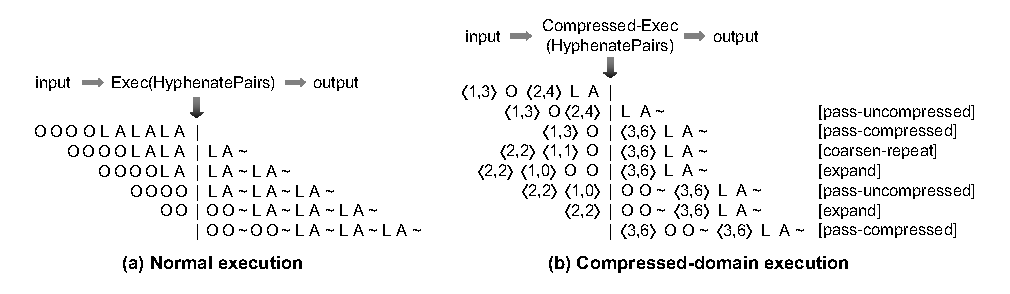
\psfig{file=compressed-filter-example.eps,width=\textwidth}
\vspace{6pt}
\caption{Example execution of a filter in the uncompressed and
  compressed domains.\protect\label{fig:filter-example}}
\end{figure*}

\begin{figure}[t]
$S \concat V \rightarrow T~~~~|V|=n$\name{exec-uncompressed} \skiptopb
---------------------------- \skipbot
$S \rightarrow F(V) \concat T$
~ \\ ~ \\
%\hfill\mbox{\it Same as above.}\name{exec-uncompressed}\vspace{6pt}\\
$S \concat \tup{d}{c} \rightarrow T~~~~d$\%$n=0~~~~c$\%$n=0$\name{exec-compressed} \skiptopb
------------------------------------------------ \skipbot
$S \rightarrow \tup{m{\x}d/n}{m{\x}c/n} \concat T$
\caption{Semantics of \textsc{Compressed-Exec(F)}: execution of filter
$F$ in the compressed domain.
%This filter also includes an {\tt exec-uncompressed} rule, which is
%identical to the one in Figure~\ref{fig:exec-rule}.
Notations are defined in Figure~\ref{fig:notations}.
\protect\label{fig:compressed-exec-rule}}
\end{figure}

Filter execution in the compressed domain requires a two-stage
transformation (see Figure~\ref{fig:actor-pic} for an overview, and
Figure~\ref{fig:filter-example} for a detailed example).  First, the
input stream is aligned to a granularity $n$ that matches the input
rate of the filter.  This alignment guarantees that every token in the
stream is either a sequence of $n$ values, or a repeat in which both
the distance and the count are multiples of $n$.  The alignment stage
(described in detail later) is a no-op for filters that pop only one
item ($n=1$).

After the alignment stage comes the execution of the compressed
filter, which appears in Figure~\ref{fig:compressed-exec-rule}.  The
{\tt exec-uncompressed} rule
%(not shown in Figure~\ref{fig:compressed-exec-rule}) 
deals with values on the input stream, and is identical to that in the
uncompressed execution.  The {\tt exec-compressed} rule deals with
repeats on the input stream and encapsulates the key idea of the
paper.  Because the inputs are repeating at the correct granularity,
the repeat can be copied directly to the output of the filter without
performing any new computation.  The only change needed is to adjust
the repeat distance and count to match the filter's output rate.

\subsubsection{Stream Alignment}

The alignment phase is needed for filters that pop more than one item
from the input stream.  Its goal is to align the execution boundaries
of the filter with the repeat boundaries of the compressed data; this
alignment is required for the compressed execution.  Following
alignment, each execution of a filter will input either $n$
consecutive values, or a repeat token with a distance and count that
are evenly divisible by $n$ (where $n$ represents the pop rate of the
filter).

The alignment stage sometimes needs to partially decompress the data
in the stream.  Due to the sliding-window dictionary in LZ77, in
general it is difficult to decode only a few items without
decompressing others.  Thus, our formulation assumes that a fully
decompressed version of the stream is available; the transition rules
access the decompressed data using the \mbox{\it decode} function,
which returns the sequence of values represented by a repeat token at
its current position in the stream.  However, in practice, this
decompression can be avoided whenever the repeat distance is the same
as the window size, as this simply causes a value in the window to be
overwritten by itself.  This case is very common in several practical
compression formats; for example, in Apple Animation, the vast
majority of repeats reference the same pixel in the previous frame
(which is also the window size), and thus most decompression is
avoided.  In run-length encoding, the repeat distance and the window
size are always equal to one, so no decompression is needed.  While
general LZ77 does require a decompressed window to be maintained, our
technique still offers significant benefits by computing on a smaller
volume of data and avoiding the cost of re-compression.  For general
algorithms such as gzip, compression can be up to 10x slower than
decompression~\cite{ziviani00compression}.

The semantics of stream alignment are given in
Figure~\ref{fig:stream-align}.  If the end of the input stream
contains $n$ values, then alignment is satisfied and the values are
moved to the output stream (rule {\tt pass-uncompressed}).  Likewise,
if the input contains a repeat in which the distance is a multiple of
$n$ and the count is at least $n$, then a number of aligned repeats
are peeled from the input and moved to the output (rule {\tt
  pass-compressed}).  If the count is not a multiple of $n$, then part
of the repeat is leftover and remains on the input stream.

There are some cases in which a repeat cannot be moved to the output
stream, in which case the data needs to be partially decompressed
(rule {\tt expand}).  This occurs if the repeat has a count less than
$n$, if it occurs in the middle of an aligned stretch of $n$ values,
or if its distance is not a multiple of $n$ (this last condition can
sometimes be remedied by another rule, see below).  The {\tt expand}
rule decodes only one value from an unaligned repeat token, thereby
decreasing its count by one; the rest of the repeat may become aligned
later.  If the count of a repeat reaches zero, it is eliminated by the
{\tt prune} rule.

\begin{figure}[t]
$S \concat V \rightarrow T~~~|V|=n$\name{pass-uncompressed}\skiptopb
---------------------------\skipbot
$S \rightarrow V \concat T$
~ \\ ~ \\
$S \concat \tup{d}{c} \rightarrow T~~~d$\%$n=0~~~c \ge n$\name{pass-compressed}\skiptopb
------------------------------------------\skipbot
$S \concat \tup{d}{c$\%$n} \rightarrow \tup{d}{c-c$\%$n} \concat T$
~ \\ ~ \\
$S \concat \tup{d}{c} \concat V \rightarrow T$\name{expand}\\
$c<n~\vee~1 \le |V|<n~\vee~(d$\%$n>0~\wedge~\neg(d < \mbox{LCM}(d,n) < c))$\skiptopb
--------------------------------------------------------------------------------\skipbot
$S \concat \tup{d}{c-1} \concat \mbox{\it decode}(\tup{d}{1}) \concat V \rightarrow T$
~ \\ ~ \\
$S \concat \tup{d}{0} \concat V \rightarrow T$\name{prune}\skiptopb
------------------------\skipbot
$S \concat V \rightarrow T$
~ \\ ~ \\
let~$L=\mbox{LCM}(d,n)$\name{coarsen-repeat}\\
$S \concat \tup{d}{c} \concat V \rightarrow T~~~~d$\%$n > 0~~~~d < L < c$\vspace{-3pt}\skiptopa
-------------------------------------------------------\skipbot
$S \concat \tup{L}{c-(L-d)} \concat \tup{d}{L-d} \concat V \rightarrow T$
\caption{Semantics of \textsc{Align}($n$): aligning data
to a granularity of $n$.  The \mbox{\it decode} function uncompresses
a repeat token into a list of values; other notations are given in
Figure~\ref{fig:notations}. \protect\label{fig:stream-align}}
\end{figure}

The final rule, {\tt coarsen-repeat}, preserves a specific kind of
compression in the input stream.  Consider that a filter pops two
items at a time, but encounters a long repeat with distance three and
count 100.  That is, the input stream contains a regular pattern of
values with periodicity three.  Though consecutive executions of the
filter are aligned at different offsets in this pattern, every third
filter execution (spanning six values) falls at the same alignment.
In general, a repeat with distance $d$ can be exploited by a filter
with pop rate $n$ by expanding the distance to $\mbox{LCM}(d, n)$.  In
order to perform this expansion, the count must be greater than the
distance, as otherwise the repeat references old data that may have no
periodicity.  Also, the stream needs to be padded with $\mbox{LCM}-d$
values before the coarsened repeat can begin; this padding takes the
form of a shorter repeat using the original distance.

%% NOTE: the second point made in this section is not quite true,
%% since you still need to decompress RLE units that are a frame away
%% in Apple Animation.  Also first point seems redundant with align
%% being no-op for pop=1, so not including this.
%%
%% \subsubsection{Optimizations}
%% \label{sec:opt}
%%
%% As the transformation to the compressed domain is formulated in
%% fully general terms, the process can be streamlined considerably for
%% common classes of inputs:
%% \begin{itemize}
%% \item If a filter has a pop rate of one ($n=1$) on a given stream then
%%   no alignment stage is needed.
%% \item If the repeat distance is equal to the LZ77 window size, then no
%%   decompression is needed because it would simply overwrite the same
%%   values in the buffer.  This property holds for inter-frame repeats
%%   in the Apple Animation format (see Section~\ref{sec:formats}).
%% \end{itemize}
%% A consequence of the first bullet is that filters with a pop rate of
%% one (such as the InvertColor filter in Figure~\ref{fig:streamit}) avoid
%% performing any decompression, as there is no alignment stage.  This
%% guarantees that the output of the filter will be the same size as the
%% compressed input.

%% \subsection{Extensions}
%% \label{sec:extensions}

%% The transformation can be extended to support a broader class of
%% filters.  Some straightforward extensions are as follows:
%% \begin{itemize}

%% \item {\it Filters with state.}  If a filter retains mutable state from
%% one execution to the next, a repeat token can be copied across the
%% filter if the current state values are the same as they were at the
%% beginning of the repeated segment.  One could maintain a lookup table
%% that tracks the state values for the sake of this comparison.  Also,
%% state updates that have a closed form can be applied in the compressed
%% domain even if the current state has never been seen before; for
%% example, if a histogram filter runs for $n$ iterations on a blue
%% pixel, it will increment the blue count by $n$ regardless of the
%% initial value.

%% \item {\it Dynamic input and output rates.}  The current formulation
%% relies on a filter's fixed I/O rates to calculate repeat distances and
%% counts for the output tape from the repeat tokens on the input tapes.
%% However, in the presence of unpredictable I/O rates (e.g., edge
%% detection), a lookup table could be used to track the actual I/O rates
%% on each execution.  In the event of a repeat, the recorded I/O rates
%% from the previous execution could be used to calculate the repeat
%% parameters on the output tape.

%% \item {\it Sliding window computations.}  We currently assume that an
%% filter consumes all of the items it inspects on a given execution step.
%% However, some filters (e.g., a Gaussian blur filter) inspect a window
%% of values in addition to the one that is consumed.  Such {\it peeking}
%% filters can be supported by adjusting the translation of repeat
%% tokens, shortening the output count to match the period that the
%% entire window was within the repeated range.

%% \end{itemize}

\subsection{Splitters}

It is necessary to consider splitters and joiners separately from
general-purpose actors because of their pass-through semantics: the
inputs are distributed to the outputs without performing any
computation.  Our translation to the compressed domain leverages this
fact to preserve considerably more compression than would be possible
if splitters and joiners were viewed as opaque computational nodes
with multiple inputs and multiple outputs.  Consequently, splitters
and joiners should be employed by the programmer not only as a natural
expression of parallelism, but as a powerful way of exposing the data
reordering to the compiler.

As mentioned previously, splitters and joiners adopt a fine-grained
cyclo-static execution model, in which each execution step transfers
only one item from an input tape to an output tape.  That is, a
roundrobin$(k_1, k_2)$ splitter or joiner has $k_1 + k_2$ distinct
execution steps.  We refer to every group of $k_1 + k_2$ steps as an
{\it execution cycle}.

Duplicate splitters are trivial to transform to the compressed domain,
as all input tokens (both values and repeats) are copied directly to
the output streams.  For roundrobin splitters, the central concern is
that a repeat token can only be transferred to a given output tape if
the items referenced are also on that tape.  If the items referenced
by the repeat token were distributed to another tape, then the repeat
must be decompressed.

\begin{figure}[t]
\vspace{-1pt} % makes a page break difference, amazing
~~~~~~~~~\psfig{figure=sj-figure.eps,width=2.8in}

\mbox{~~~~~~~~~~}(a) Notation for splitters~~~~~~~~~~~~~~(b) Notation for joiners
\caption{Notations used in the semantics for splitters and joiners.
  In addition, the variable $\pos$ indicates how many items have been
  written to (in the case of splitters) or read from (in the case of
  joiners) the active tape during the current execution cycle.
  \protect\label{fig:sj-pic}}
\end{figure}

The rest of this section focuses on roundrobin splitters.  To simplify
the presentation, we consider a splitter with only two output streams.
This captures all of the fundamental ideas; extension to additional
streams is straightforward.  Rewrite rules now take the following
form:

\hspace{-12pt}\begin{tabular}{l} ~ \vspace{-6pt} \\ 
\hspace{-3pt}$S \rightarrow T_1; T_2$ \hspace{-7pt}~\vspace{0.5pt} \\ \hline ~ \vspace{-7.5pt} \\
\hspace{-3pt}$S' \rightarrow T_1'; T_2'$ \hspace{-7pt} \\ ~ \vspace{-6pt} \\
\end{tabular}

\noindent where $T_1$ and $T_2$ represent the output streams of the
splitter (see Figure~\ref{fig:sj-pic}).  In addition, we make two
further simplifications:
\begin{itemize}

\item The rules assume that the next execution step of the splitter
  will write to $T_1$.  The subscripts should be interpreted without
  loss of generality.

\item We use $\pos$ to denote the number of items (in terms of the
  uncompressed domain) that have already been written to the current
  output stream ($T_1$) in the current execution cycle.  For brevity,
  the rules do not maintain the value of $\pos$, though it is
  straightforward to do so.

\end{itemize}

The semantics for splitter execution in the uncompressed domain appear
in Figure~\ref{fig:uncompressed-splitter}.  The {\tt
  pass-uncompressed} rule simply passes a single value from the input
tape to the current output tape, $T_1$.  Note that the current
position $\pos$ is implicitly incremented; once $\pos$ reaches $m_1$,
it is reset to zero and the output tapes are switched (tape $T_2$ will
be named $T_1$ on the next execution).

The compressed-domain semantics for splitters are given in
Figure~\ref{fig:compressed-splitter}, and a detailed example appears
in Figure~\ref{fig:sj-example}.  As mentioned previously, a repeat
token can be transferred to an output tape so long as the items
referenced also appear on that tape.  However, the repeat may need to
be fragmented (into several repeats of a lesser count), depending on
the repeat distance.  There are two cases to consider.

\begin{figure}[t]
$S \concat V \rightarrow T_1; T_2~~~~|V|=1$\name{pass-uncompressed}\skiptopb
---------------------------------\skipbot
$S \rightarrow V \concat T_1; T_2$
\caption{Semantics of \textsc{Splitter}: execution of a roundrobin
  splitter in the uncompressed domain.
 \protect\label{fig:uncompressed-splitter}}
\end{figure}

\begin{figure}[t]
$S \concat V \rightarrow T_1; T_2~~~~|V|=1$\name{pass-uncompressed}\skiptopb
---------------------------------\skipbot
$S \rightarrow V \concat T_1; T_2$
~ \\ ~ \\
let~$\mbox{offset} = d$\%$(m_1+m_2)$\name{pass-compressed-long}\skiptopb
let~$(L_1, L_2) = \mbox{run\_splitter}(c)$\vspace{2pt}\\
$S \concat \tup{d}{c} \rightarrow T_1; T_2~~~~\mbox{offset} = 0$\vspace{-3pt}\skiptopa
--------------------------------------------\skipbot
$S \rightarrow \tup{d{\x}m_1/(m_1+m_2)}{L_1} \concat T_1;$\\
\mbox{~~~~~~~~~}\hspace{0.29pt}$\tup{d{\x}m_2/(m_1+m_2)}{L_2} \concat T_2$
~ \\ ~ \\
let~$\mbox{offset} = d$\%$(m_1+m_2)$\name{pass-compressed-short}\skiptopb
let~$\mbox{offset'} = \mbox{\bf if~} \mbox{offset} \leq \pos \mbox{\bf ~then~} \mbox{offset}$\\
\mbox{~}\hspace{42.3pt}$\mbox{\bf ~else~} \mbox{offset} - m_2$\\
let~$\mbox{actual\_repeat} = \mbox{min}(c, \mbox{split\_potential}(d))$\\
$S \concat \tup{d}{c} \rightarrow T_1; T_2~~~~\mbox{offset} > 0~~~~\mbox{split\_potential}(d) > 0$\skiptopb
-------------------------------------------------------------------------\skipbot
$S \concat \tup{d}{c - \mbox{actual\_repeat}} \rightarrow$\\
$\tup{m_1*\mbox{floor}(d / (m_1 + m_2)) + \mbox{offset'}}{\mbox{actual\_repeat}} \concat T_1; T_2$
~ \\ ~ \\
let~$\mbox{offset} = d$\%$(m_1+m_2)$\name{expand}\skiptopb
$S \concat \tup{d}{c} \rightarrow T_1; T_2~~\hspace{1pt}\mbox{offset} > 0~~\hspace{1pt}\mbox{split\_potential}(d) = 0$\skiptopb
-------------------------------------------------------------------\skipbot
$S \concat \tup{d}{c-1} \concat \mbox{\it decode}(\tup{d}{1}) \rightarrow T_1; T_2$
~ \\ ~ \\
$S \concat \tup{d}{0} \rightarrow T_1; T_2$\name{prune}\skiptopb
------------------------\skipbot
$S \rightarrow T_1; T_2$
\caption{Semantics of \textsc{Compressed-Splitter}:  execution of a roundrobin
splitter in the compressed domain.
\protect\label{fig:compressed-splitter}}
\end{figure}

% improve this explanation
The first case, expressed by the {\tt pass-compressed-long} rule in
Figure~\ref{fig:compressed-splitter}, distributes an entire repeat
token to both output tapes without any fragmentation.  This is only
possible when the repeat can be cleanly separated into two independent
sequences, one offset by $m_1$ and the next offset by $m_2$.  In other
words, the repeat distance must be a multiple of $m_1+m_2$.  In this
case, the repeat token is moved to the output streams.  The repeat
distance is scaled down to match the weight of each stream, and the
count is divided according to the current position of the splitter (a
simple but tedious calculation implemented by {\tt run\_splitter} in
Figure~\ref{fig:helper-splitter}).

\begin{figure*}[t]
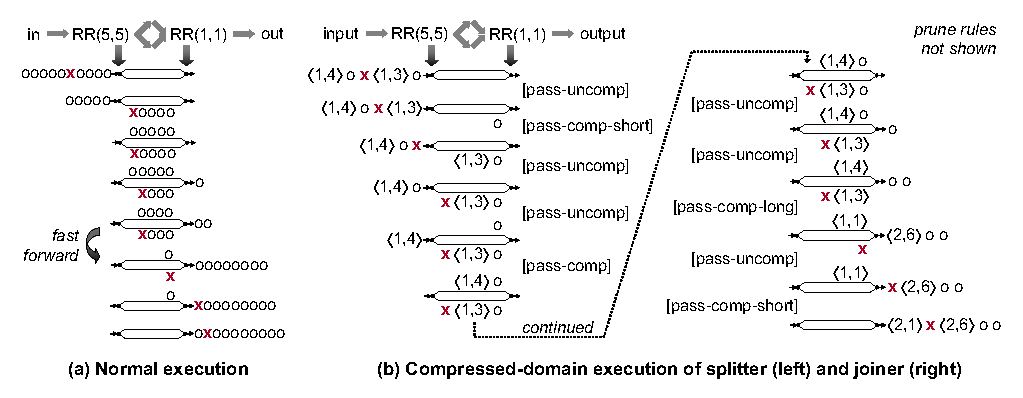
\psfig{file=compressed-splitjoin-example.eps,width=\textwidth}
\vspace{6pt}
\caption{Example execution of splitters and joiners in the compressed
  domain.  As illustrated by the input/output pairs in (a), the
  example performs a transpose of a 2x5 matrix.  When the matrix is
  linearized (as in (b) and (c)), the input stream traverses the
  elements row-wise while the output stream traverses column-wise.
  Due to redundancy in the matrix, this reordering can be done largely
  in the compressed domain.  \protect\label{fig:sj-example}}
\end{figure*}

\begin{figure}[t]
\begin{minipage}{0.1in}
\vspace{-1.75pt}
{\it // // // // //}
\end{minipage}
\begin{minipage}{3.23in}
{\it Given that $c$ items are available on input stream of a splitter,
  returns the number of items that can be written to each output stream
  before the input is exhausted.
  Assumes that the splitter is currently writing to the first output
  stream, to which \mbox{pos} items have previously been written in
  the current execution cycle.}
\end{minipage}
\mbox{\bf run\_splitter}$(c, \pos )$~returns~(int,~int)~\{\\
\tab{\it // the number of complete splitter cycles, and the leftover}\\
\tab$\mbox{total\_cycles} = \mbox{floor}(c/(m_1 + m_2))$\\
\tab$\mbox{total\_leftover} = c$\%$(m_1 + m_2)$\\
~ \vspace{-6pt}\\ 
\tab{\it // the last partial cycle may end in three regions:}\\
\tab$\mbox{\bf if~} \mbox{total\_leftover} \leq m_1 - \pos$~\{\\
\tab\tab{\it // 1. in writing to the first output stream}\\
\tab\tab$L_1 = \mbox{total\_leftover}$\\
\tab\tab$L_2 = 0$\\
\tab$\} \mbox{\bf~else if~} \mbox{total\_leftover} \leq m_1-\pos + m_2~\{$\\
\tab\tab{\it // 2. in subsequent writing to the second output stream}\\
\tab\tab$L_1 = m_1-\pos$\\
\tab\tab$L_2 = \mbox{total\_leftover} - m_1-\pos$\\
\tab\} \mbox{\bf else} \{\\
\tab\tab{\it // 3. in wrap-around writing to the first output stream}\\
\tab\tab$L_1 = \mbox{total\_leftover} - m_2$\\
\tab\tab$L_2 = m_2$\\
\tab\}\\
~ \vspace{-6pt}\\
\tab$\mbox{\bf return~}(m_1*\mbox{total\_cycles} + L_1, m_2*\mbox{total\_cycles} + L_2)$
\}\\
~ \\
\begin{minipage}{0.1in}
\vspace{-1.75pt}
{\it // // // // //}
\end{minipage}
\begin{minipage}{3.23in}
{\it Given a repeat token with distance $d$ that is input to a
  splitter, returns the maximum count of a repeat token that could
  safely be emitted to the current output stream of the splitter.
  Assumes that only a single repeat token can be emitted (i.e., the
  {\tt pass-compressed-long} rule does not apply).}
\end{minipage}
\mbox{\bf split\_potential}$(d)$~returns~int~\{\\
\tab$\mbox{offset} = d$\%$(m_1 + m_2)$\\
\tab$\mbox{{\bf if~}} \mbox{offset} \leq \pos ~\{$\\
\tab\tab{\it // repeat for remainder of this execution cycle}\\
\tab\tab$\mbox{\bf return~} m_1 - \pos$\\
\tab$\} \mbox{\bf ~else if~} \mbox{offset} > m_2 + \pos ~\{$\\
\tab\tab{\it // repeat until referenced data goes out of range}\\
\tab\tab$\mbox{\bf return~} \mbox{offset} - (m_2 + \pos)$\\
\tab$\} \mbox{\bf ~else} ~\{$\\
\tab\tab{\it // referenced data is on the other output stream}\\
\tab\tab$\mbox{\bf return~} 0$\\
\tab$\}$\\
\}
\caption{Helper functions for \textsc{Compressed-Splitter}.
\protect\label{fig:helper-splitter}}
\end{figure}

The second case, handled by the {\tt pass-compressed-short} rule, is
when the repeat distance is mis-aligned with the splitter's execution
cycle, and thus the repeat (if it is long enough) eventually
references items that are distributed to a different output tape.
Nonetheless, part of the repeat may be eligible to pass through, so
long as the items referenced refer to the current output tape.  This
judgment is performed by {\tt split\_potential}
(Figure~\ref{fig:helper-splitter}) by comparing the repeat distance to
the current position in the output stream.  If one or more of the
repeated values are in range, the valid segment of the repeat (of
length {\tt actual\_repeat}) is moved to the output tape.  As before,
the repeat distance needs to be scaled according to the weights of the
splitter, and an extra offset is needed if the repeat distance wraps
around to reference the end of a previous cycle.

If neither of the above transfers apply, then the input stream needs
to be partially decompressed (according to the {\tt expand} rule)
because the current repeat token references items that will be sent to
the wrong output tape.  The {\tt prune} rule is also needed to clear
empty repeats generated by {\tt expand}.

Though we omit the details, it is also desirable to employ an analog
of the {\tt coarsen-repeat} rule (Figure~\ref{fig:stream-align}) to
preserve even more compression across a splitter.  The intuition is
that, by increasing certain repeat distances, the splitter's output
tapes can become more independent (referencing themselves rather than
each other).  This enables a compressed rule to fire in place of an
expansion step.

\subsection{Joiners}

Analogously to splitters, there are two ways to pass repeat tokens
through a joiner.  If the input streams contain compatible repeat
tokens, then they can be combined into a long repeat that spans
multiple execution cycles; otherwise, a shorter repeat is extracted
from only one of the streams.  Both of these cases are illustrated by
example in Figure~\ref{fig:sj-example}.  Unlike splitters, there is
never a need to decompress repeat tokens into values before passing
through a joiner.  Though the repeat length may shrink to one, it will
remain a reference to a previous item rather than becoming a value
itself.

In the uncompressed domain, joiners have the semantics given in
Figure~\ref{fig:uncompressed-joiner}.  The {\tt pass-uncompressed}
rule passes a single value from the current input tape ($S_1$) to the
output tape.  Analogously to splitters, the variable $\pos$ represents
the number of items that have been read from the current input tape
and is implicitly updated.  Once $\pos$ reaches $n_1$, it is reset to
zero and the input tapes are switched (tape $S_2$ will be named $S_1$
on the next execution).

The first and most powerful way to execute joiners in the compressed
domain is to combine repeat tokens from both input streams
%
\clearpage\noindent\clearpage\noindent % WTF - with just 1 it gets really weird!
%
(rule {\tt pass-compressed-long} in
Figure~\ref{fig:compressed-joiner}).  For this to be possible, both
repeat distances must be the same multiple of their respective joiner
weight ($n_1$ or $n_2$); the combined token has a repeat distance that
is a multiple of $n_1 + n_2$.  The {\tt repeat\_lengths} routine
(Figure~\ref{fig:helper-joiner}) calculates the maximum repeat length
depending on the current position of the joiner and the repeat lengths
of the inputs.

\begin{figure}[t]
$S_1 \concat V; S_2 \rightarrow T~~~~|V|=1$\name{pass-uncompressed}\skiptopb
---------------------------------\skipbot
$S_1; S_2 \rightarrow V \concat T$
\caption{Semantics of \textsc{Joiner}: execution of a roundrobin
  joiner in the uncompressed domain.
\protect\label{fig:uncompressed-joiner}}
\end{figure}

\begin{figure}
$S_1 \concat V; S_2 \rightarrow T~~~~|V|=1$\name{pass-uncompressed}\skiptopb
---------------------------------\skipbot
$S_1; S_2 \rightarrow V \concat T$
~ \\ ~ \\
let~$(L_1, L_2) = \mbox{repeat\_lengths}(c_1, c_2, pos)$\name{pass-compressed-long}\skiptopb
$S_1 \concat \tup{d_1}{c_1};$\\
$S_2 \concat \tup{d_2}{c_2} \rightarrow T~~~~d_1$\%$n_1=0~~~~d_2$\%$n_2=0~~~~d_1/n_1=d_2/n_2$\vspace{-3pt}\skiptopa
--------------------------------------------------------------------------------\skipbot
$S_1 \concat \tup{d_1}{c_1-L_1};$\\
$S_2 \concat \tup{d_2}{c_2-L_2} \rightarrow \tup{d_1(n_1+n_2)/n_1}{L_1+L_2} \concat T$
~ \\ ~ \\
let~$\mbox{offset'} = \mbox{\bf ~if~} d$\%$n_1 \leq \pos \mbox{\bf ~then~} \pos$\name{\hspace{-0.5pt}pass-compressed-short\hspace{1.5pt}(a)\hspace{-0.5pt}}\skiptopb
$\mbox{~~~~}\hspace{37.7pt}\mbox{\bf ~else~} d$\%$n_1 + n_2$\\
let~$L=\mbox{min}(c,\mbox{join\_potential}(d))$\\
$S_1 \concat \tup{d}{c}; S_2 \concat V \rightarrow T$\vspace{-3pt}\skiptopa
--------------------------------------------------\skipbot
$S_1 \concat \tup{d}{c-L}; S_2 \concat V \rightarrow$\\
$\tup{(n_1 + n_2){\x}\mbox{floor}(d/n_1) + \mbox{offset'}}{L} \concat T$
~ \\ ~ \\
let~$\mbox{offset'} = \mbox{\bf ~if~} d$\%$n_1 \leq \pos \mbox{\bf ~then~} \pos$\name{\hspace{-0.7pt}pass-compressed-short\hspace{1.5pt}(b)\hspace{-0.7pt}}\skiptopb
$\mbox{~~~~}\hspace{37.7pt}\mbox{\bf ~else~} d$\%$n_1 + n_2$\\
let~$L=\mbox{min}(c,\mbox{join\_potential}(d))$\\
$S_1 \concat \tup{d}{c}; S_2 \concat \tup{d_2}{c_2} \rightarrow T~~~~d_2$\%$n_2 > 0$\vspace{-3pt}\skiptopa
-------------------------------------------------------\skipbot
$S_1 \concat \tup{d}{c-L}; S_2 \concat \tup{d_2}{c_2} \rightarrow$\\
$\tup{(n_1 + n_2){\x}\mbox{floor}(d/n_1) + \mbox{offset'}}{L} \concat T$
\\ ~ \\
$S_1 \concat \tup{d}{0}; S_2 \rightarrow T$\name{prune}\skiptopb
------------------------\skipbot
$S_1; S_2 \rightarrow T$
\caption{Semantics of \textsc{Compressed-Joiner}.
\protect\label{fig:compressed-joiner}}
\end{figure}

\begin{figure}[t]
\begin{minipage}{0.1in}
\vspace{-1.75pt}
{\it // // // // // //}
\end{minipage}
\begin{minipage}{3.23in}
{\it Given that $c_1$ and $c_2$ items are available on the first and
  second input streams of a joiner, returns the number of items that
  can be read from each input before one of them is exhausted.
  Assumes that the joiner is currently reading from the first input
  stream, from which \mbox{pos} items have previously been consumed in
  the current execution cycle.}
\end{minipage}
\mbox{\bf repeat\_lengths}$(c_1, c_2, \pos )$~returns~(int,~int)~\{\\
\tab{\it // the number of complete joiner cycles, and the leftovers}\\
\tab$\mbox{total\_cycles} = \mbox{floor}(c/(n_1 + n_2))$\\
\tab$\mbox{leftover}_1 = c_1 - \mbox{total\_cycles} * n_1$\\
\tab$\mbox{leftover}_2 = c_2 - \mbox{total\_cycles} * n_2$\\
~ \vspace{-6pt}\\
\tab{\it // the last partial cycle may end in three regions:}\\
\tab$\mbox{\bf if~} \mbox{leftover}_1 \leq n_1 - \pos$~\{\\
\tab\tab{\it // 1. in reading from the first input stream}\\
\tab\tab$L_1 = \mbox{leftover}_1$\\
\tab\tab$L_2 = 0$\\
\tab$\} \mbox{\bf~else if~} \mbox{leftover}_2 \leq n_2~\{$\\
\tab\tab{\it // 2. in subsequent reading from the second input stream}\\
\tab\tab$L_1 = n_1-\pos$\\
\tab\tab$L_2 = \mbox{leftover}_2$\\
\tab\} \mbox{\bf ~else} \{\\
\tab\tab{\it // 3. in wrap-around reading from the first input stream}\\
\tab\tab$L_1 = \mbox{leftover}_1$\\
\tab\tab$L_2 = n_2$\\
\tab\}\\
~ \vspace{-6pt}\\ 
\tab$\mbox{\bf return~}(n_1*\mbox{total\_cycles} + L_1, n_2*\mbox{total\_cycles} + L_2)$
\}\\
~ \\
\begin{minipage}{0.1in}
\vspace{-1.75pt}
{\it // // // // //}
\end{minipage}
\begin{minipage}{3.23in}
{\it Given a repeat token with distance $d$ on the current input
  stream of a joiner, returns the maximum count of a repeat token that
  could safely be emitted to the output stream.  Assumes that only a
  single repeat token is available (i.e., the {\tt
    pass-compressed-long} rule does not apply).}
\end{minipage}
\mbox{\bf join\_potential}$(d)$~returns~int~\{\\
\tab$\mbox{offset} = d$\%$n_1$\\
\tab$\mbox{{\bf if~}} \mbox{offset} \leq \pos ~\{$\\
\tab\tab{\it // repeat for remainder of this execution cycle}\\
\tab\tab$\mbox{\bf return~} n_1 - \pos$\\
\tab$\} \mbox{\bf ~else} ~\{$\\
\tab\tab{\it // repeat until referenced data goes out of range}\\
\tab\tab$\mbox{\bf return~} \mbox{offset} - \pos$\\
\tab$\}$\\
\}
\caption{Helper functions for \textsc{Compressed-Joiner}.
\protect\label{fig:helper-joiner}}
\end{figure}

The second mode of compressed joiner execution inputs only a single
repeat token, extracting the maximum length that can safely move to
the output.  This rule is needed when the previous one does not apply:
if the second stream ends in a value rather than a repeat ({\tt
  pass-compressed-short (a)}) or the repeat distance has the wrong
granularity ({\tt pass-compressed-short (b)}).  The {\tt
  join\_potential} routine (Figure~\ref{fig:helper-joiner}) determines
how much of the repeat can be moved to the output before the data
referenced would have originated from a different input stream.

As in the case of splitters, further compression gains are possible by
adding rules to coarsen the repeat distance or shift the distance to
align with other streams.  We omit the details here.

%\section{Supported File Formats}
\label{sec:formats}

As LZ77 refers to a compression algorithm rather than a complete
compression format, there are additional factors to consider in
mapping computations to real-world image and video codecs.  Some
codecs are a subset of LZ77, utilizing only run-length encoding or a
fixed window size; these are supported very efficiently by our
technique.  Others are a superset of LZ77, incorporating additional
techniques such as delta coding or Huffman coding; these may incur
additional processing overhead.  In the following sections, we
describe the practical considerations involved in targeting various
compression formats with our technique.
%Formats are ordered by approximate goodness of the achievable mapping.

\subsection{High-Efficiency Mappings}
\label{sec:formats-good}

All of the formats in this category can be considered to be subsets of
LZ77.

\paragraph{Apple Animation.}  
The Apple Animation codec (which forms the basis for our experimental
evaluation) is supported as part of the Quicktime MOV container
format.  It serves as an industry standard for exchanging computer
animations and digital video content before they are rendered to lossy
formats for final distribution~\cite[p.~106]{adobe-anim}\cite[p.~284]{harrington-anim} \cite[p.~367]{long-anim}\cite[p.~280]{pogue-anim}.

The Animation codec represents a restricted form of LZ77 in which
repeat distances are limited to two values: a full frame or a single
pixel.  A repeat across frames indicates that a stretch of pixels did
not change from one frame to the next, while a repeat across pixels
indicates that a stretch of pixels has the same color within a frame.
% mention bit depths?

\begin{table*}[t]
\vspace{-1\baselineskip}
\psfig{figure=table-benchmarks.eps,width=7.1in}
\caption{Characteristics of the video workloads.
\protect\label{tab:videos}}
\end{table*}

\paragraph{Flic Video.}
Flic Video files (FLI/FLC) were originally produced by Autodesk
Animator and are still supported by many animation packages today.
Their compression of frame data is almost identical to Apple
Animation.

\paragraph{Microsoft RLE.}
Microsoft RLE compression can appear in both BMP images and AVI
animations.  Apart from bit-depth and formatting details, its
capabilities are identical to Apple Animation; it can perform
run-length encoding within a frame, and can skip over pixels to
exploit inter-frame redundancy.

\paragraph{Targa.}
The Truevision Targa (TGA) format is a simple image format that is
widely used to render frame sequences in the computer animation and
video industries.  The format includes an optional RLE compression
stage, making it a good target for our technique.

%% \paragraph{PXY.}
%% The pxy format is a research-based image format designed to support
%% efficient transpose and rotation of black-and-white
%% images~\cite{shoji95}.  It consists of the series of $(x,y)$
%% coordinates at which the image changes color during a horizontal scan.
%% As this information can be converted to a run-length encoding, it can
%% also be targetted by our technique.

%% \subsection{Medium-Efficiency Mappings}
%% \label{sec:formats-med}

%% While the formats in this category utilize an encoding that is
%% compatible with LZ77, they incur extra overhead because the data is
%% reorganized prior to the compression stage.

%% \paragraph{Planar RGB.}
%% The Planar RGB video format is supported by Apple Quicktime files.  It
%% utilizes run-length encoding for pixels within a frame, with partial
%% support for expressing inter-frame repeats (only the end of lines can
%% be skipped).  The red, green, and blue planes are encoded separately
%% in order to increase compression.  For user transformations that need
%% to process red, green, and blue values together, this introduces
%% additional alignment overhead when applying our technique.

%% \paragraph{OpenEXR.}
%% OpenEXR is an emerging image format (backed by Industrial Light and
%% Magic) for use in digital film.  It offers several compression
%% options, including run-length encoding, zip, and wavelet-based
%% compression.  However, in run-length encoding mode, the low and high
%% bytes of the pixels are separated and encoded as separate run-length
%% sequences; this enables pixels with variations in the low bytes to
%% nonetheless benefit from compression of the high bytes.  As most user
%% transformations would utilize the entire bit-width of the pixel, our
%% technique suffers additional alignment overhead in processing these
%% files.

\subsection{Low-Efficiency Mappings}
\label{sec:formats-bad}

The formats in this category are supersets of LZ77.  While our
technique could offer some gains in exploiting the LZ77 compression,
it would have to undo any compression sitting on top of LZ77 and
offers limited benefit for filters (as in PNG) applied underneath
LZ77.

\paragraph{DEFLATE.}
DEFLATE is a general-purpose algorithm that provides all of the
compression for popular formats such as ZIP and GZIP.  The algorithm
consists of a full LZ77 encoder followed by Huffman coding, which
resizes the symbols in the stream to match their usage frequencies.
In targeting ZIP or GZIP with our transformations, we would first
have to undo the Huffman coding (unless the application simply
reordered data, in which case the coding could remain intact).  Though
Huffman decoding is a lightweight lookup operation, it would also
increase the memory footprint.  In addition, as DEFLATE's LZ77
algorithm operates on individual bytes, there may be an exaggerated
alignment cost if the application operates on a larger word size.

%% \paragraph{TSCC.}
%% The TechSmith Screen Capture Codec is very similar to Microsoft RLE,
%% except that the final output is further compressed using DEFLATE.
%% Thus, any overheads incurred by our technique on DEFLATE also extend
%% to TSCC.

\paragraph{PNG.}
The PNG image format also relies on DEFLATE to compress the pixels in
the image.  However, before running DEFLATE, the pixels are usually
filtered with a delta encoding; each pixel is replaced with the
difference between its value and a predicted value, where the
prediction is a linear combination of neighboring pixels.  While
program segments that compute a linear function~\cite{aalamb} could
perhaps be mapped to this compressed format, our current technique
only applies if the delta encoding is turned off.  Even in this
scenario, there is a large amount of overhead due to the Huffman
coding in DEFLATE.

\section{Evaluation}
\label{sec:eval}

In this section we evaluate the framework presented in this paper.  We
have implemented the techniques in the context of the StreamIt
compiler infrastructure~\cite{gordon-asplos06}.  The fission and
sharing reduction techniques are guided by the parallelization
management algorithms covered in~\cite{gordon-asplos06}.  These
algorithms offer a holistic approach to exploiting coarse-grained
task, data, and pipeline parallelism.   Once, the parallelization management
algorithm decides how to exploit data-parallelism, i.e., which
filters should be data parallelized and by what degree, our fission
algorithm of Section~\ref{sec:data-par} is utilized to perform the
data-parallelization. 

We compare our techniques to previously published techniques for
fission of sliding window filters that perform duplication of all
input items and decimation of unneeded items (DupDec).  We employ
three benchmarks for the evaluation.  The ChannelVocoder benchmark is
the analyzer portion of a source-filter model speech coder.  The
Filterbank benchmark implements a multi-rate signal decomposition
processing block common in communications and image processing.  The
FMRadio benchmark implements an FM radio with multi-band equalizer.
The following table provides more details on the benchmarks:


{\centering
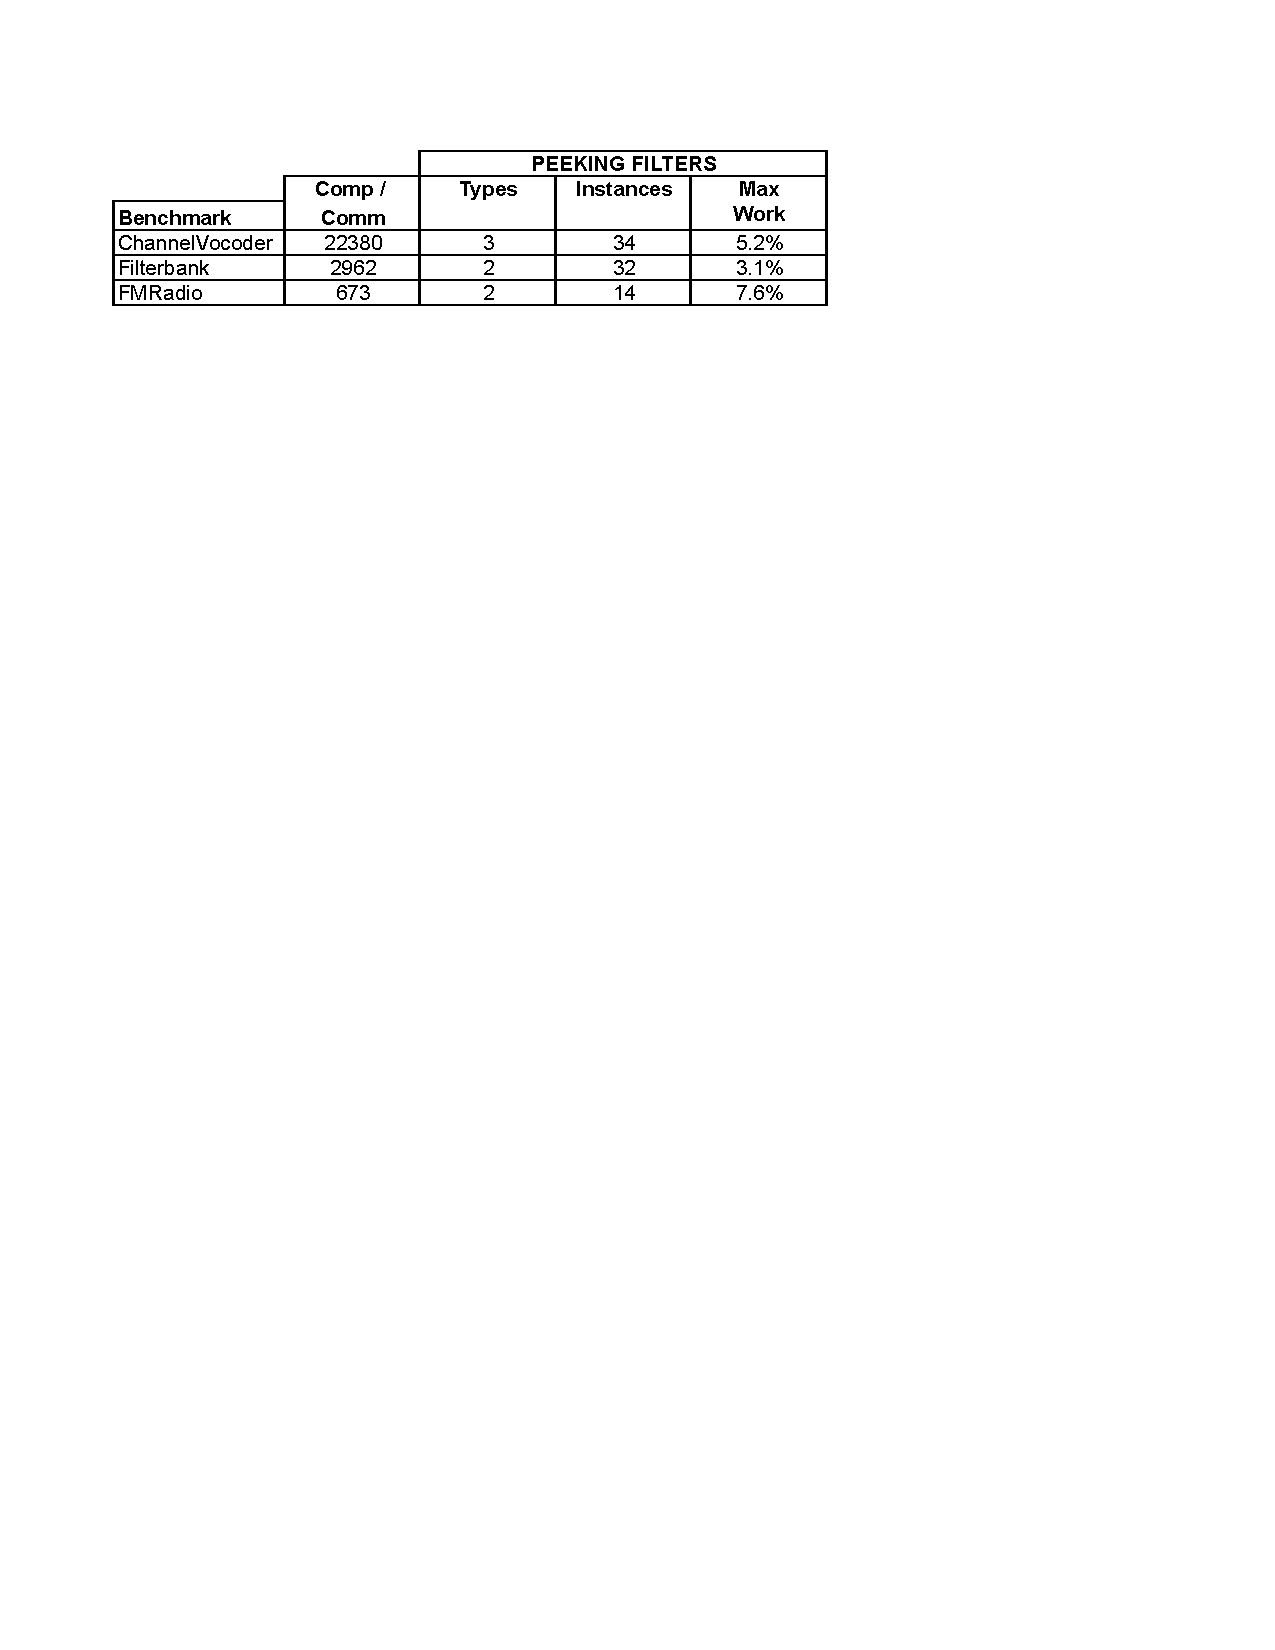
\includegraphics[width=3.3in]{figures/bench-char.pdf}}

\noindent ``Comp/Comm'' provides a static estimation of the
amount of computation to communication ratio by statically estimating the total
work of all the filters and dividing by the number items communicated
for the programmer-conceived graph's steady-state.  The remaining
statistics give the number of peeking filters types, number of peeking
filters instantiated at runtime, and a static estimation of the maximum
work in the single most loaded peeking filter.

We target 2 multicore architecture with different communication
mechanisms.  The Tilera Corporation's TILE64 Processor is a 64 core
system on a chip~\cite{tilera}.  Each core is an identical three-wide
VLIW. The code generated by the StreamIt
compiler for the TILE64 processor follows the remote store programming
(RSP) model~\cite{rsp10} in which each process has a private address
space, but each process can award remote processes write access to
their local memory. When a producer process has write access to a
consumer process's memory, the producer communicates directly with the
consumer via store instructions whose destination is an address in the
consumer's shared memory.  Communication is initiated by the producer,
and is fine-grained.  The consumer reads directly from it's local
memory (L2) when accessing input.

Our symmetric multiprocessor target is a 16-core architecture that is
comprised of four Intel Xeon E7350 multicore processors.  Each processor
is a 64-bit, quad-core with two dual-core dies.  Each die contains a 4
MB L2 cache shared across the two cores.  The front-side bus is clocked
at 1066 MHz.  We utilize the cache coherency mechanism of the
architecture for communication between cores. 

Through empirical experimentation on FMRadio, Filterbank, and
ChannelVocoder, we have settled on $T_{\mt{sharing}} =.10$ and
$T_{\mt{apply}} = 0.05$. These constants are the sweet stop for the two
architectures employed in the experimentation, being a good compromise
between buffer size and inter-core communication.

% \begin{figure*}[t]
% \centering
% \subfigure[]{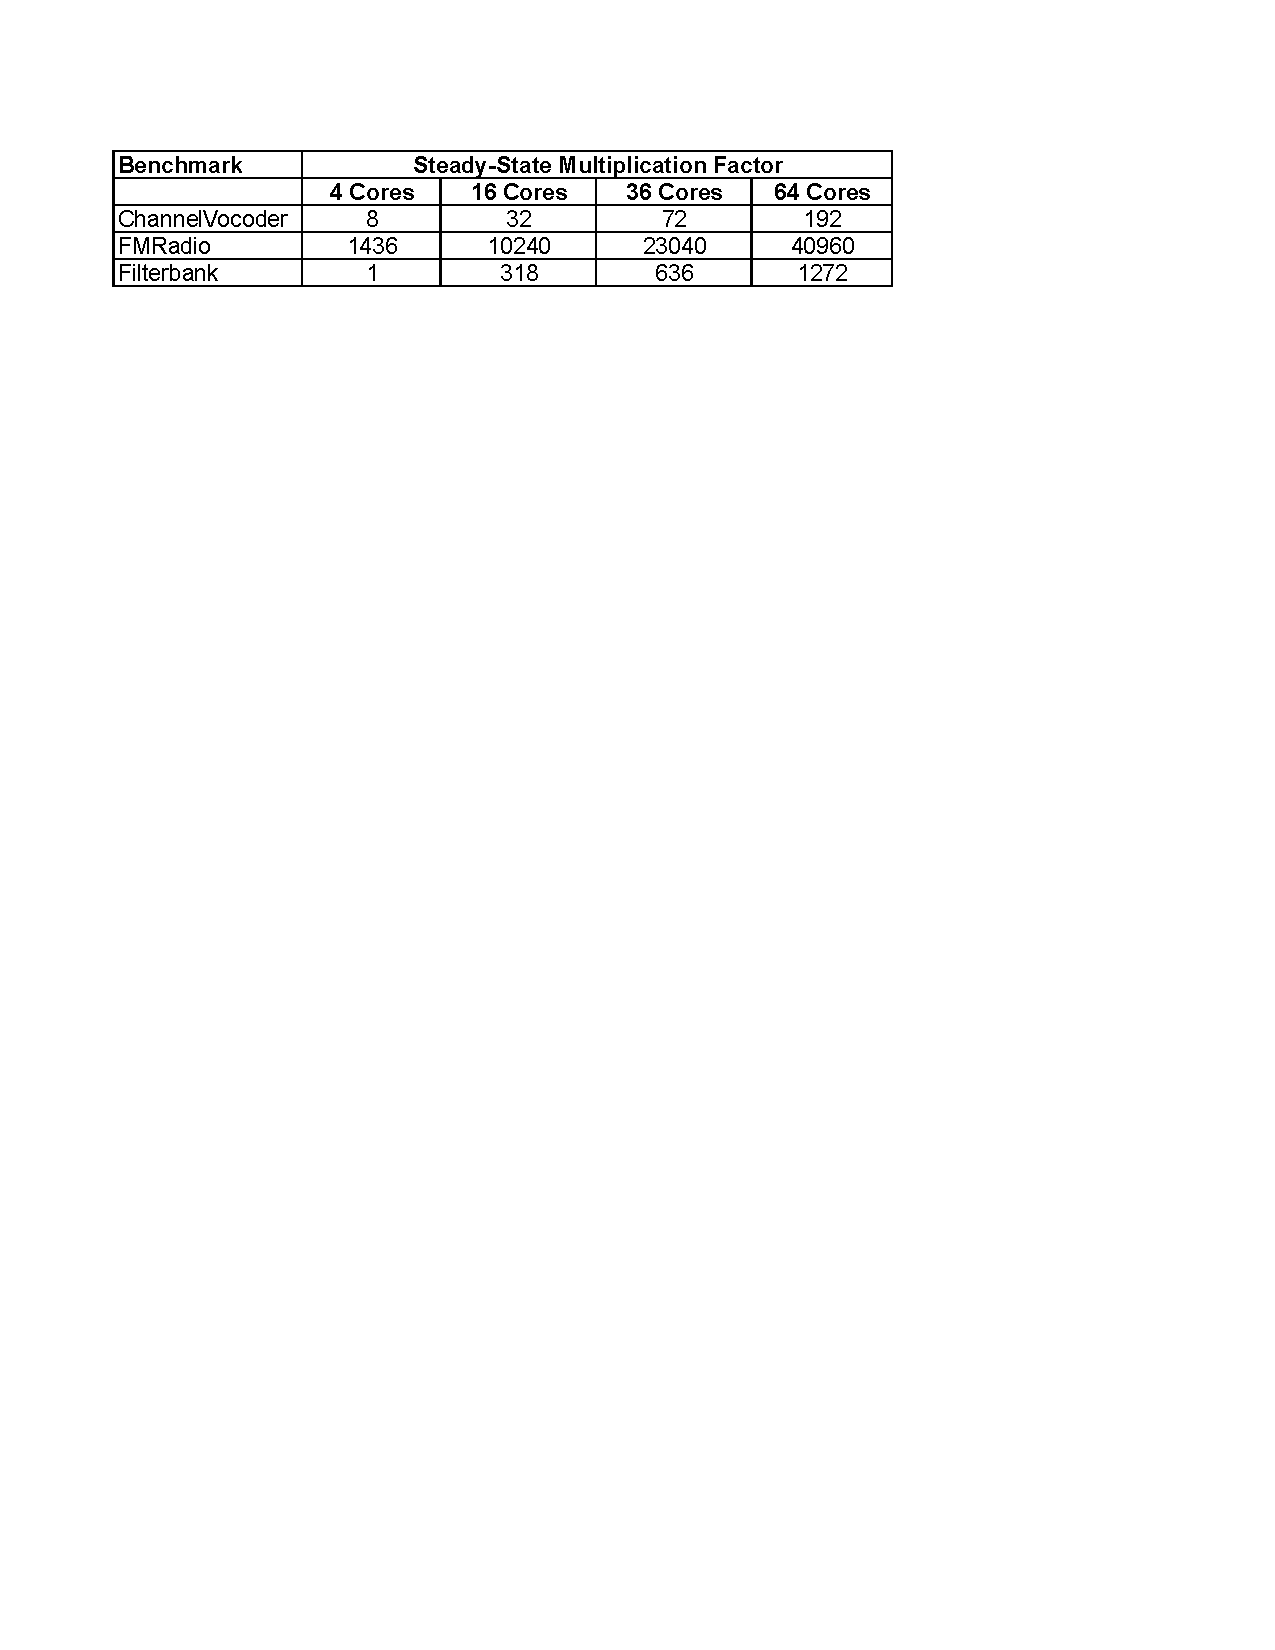
\includegraphics[width=3.7in]{figures/mult-table.pdf}} \\
% \subfigure[]{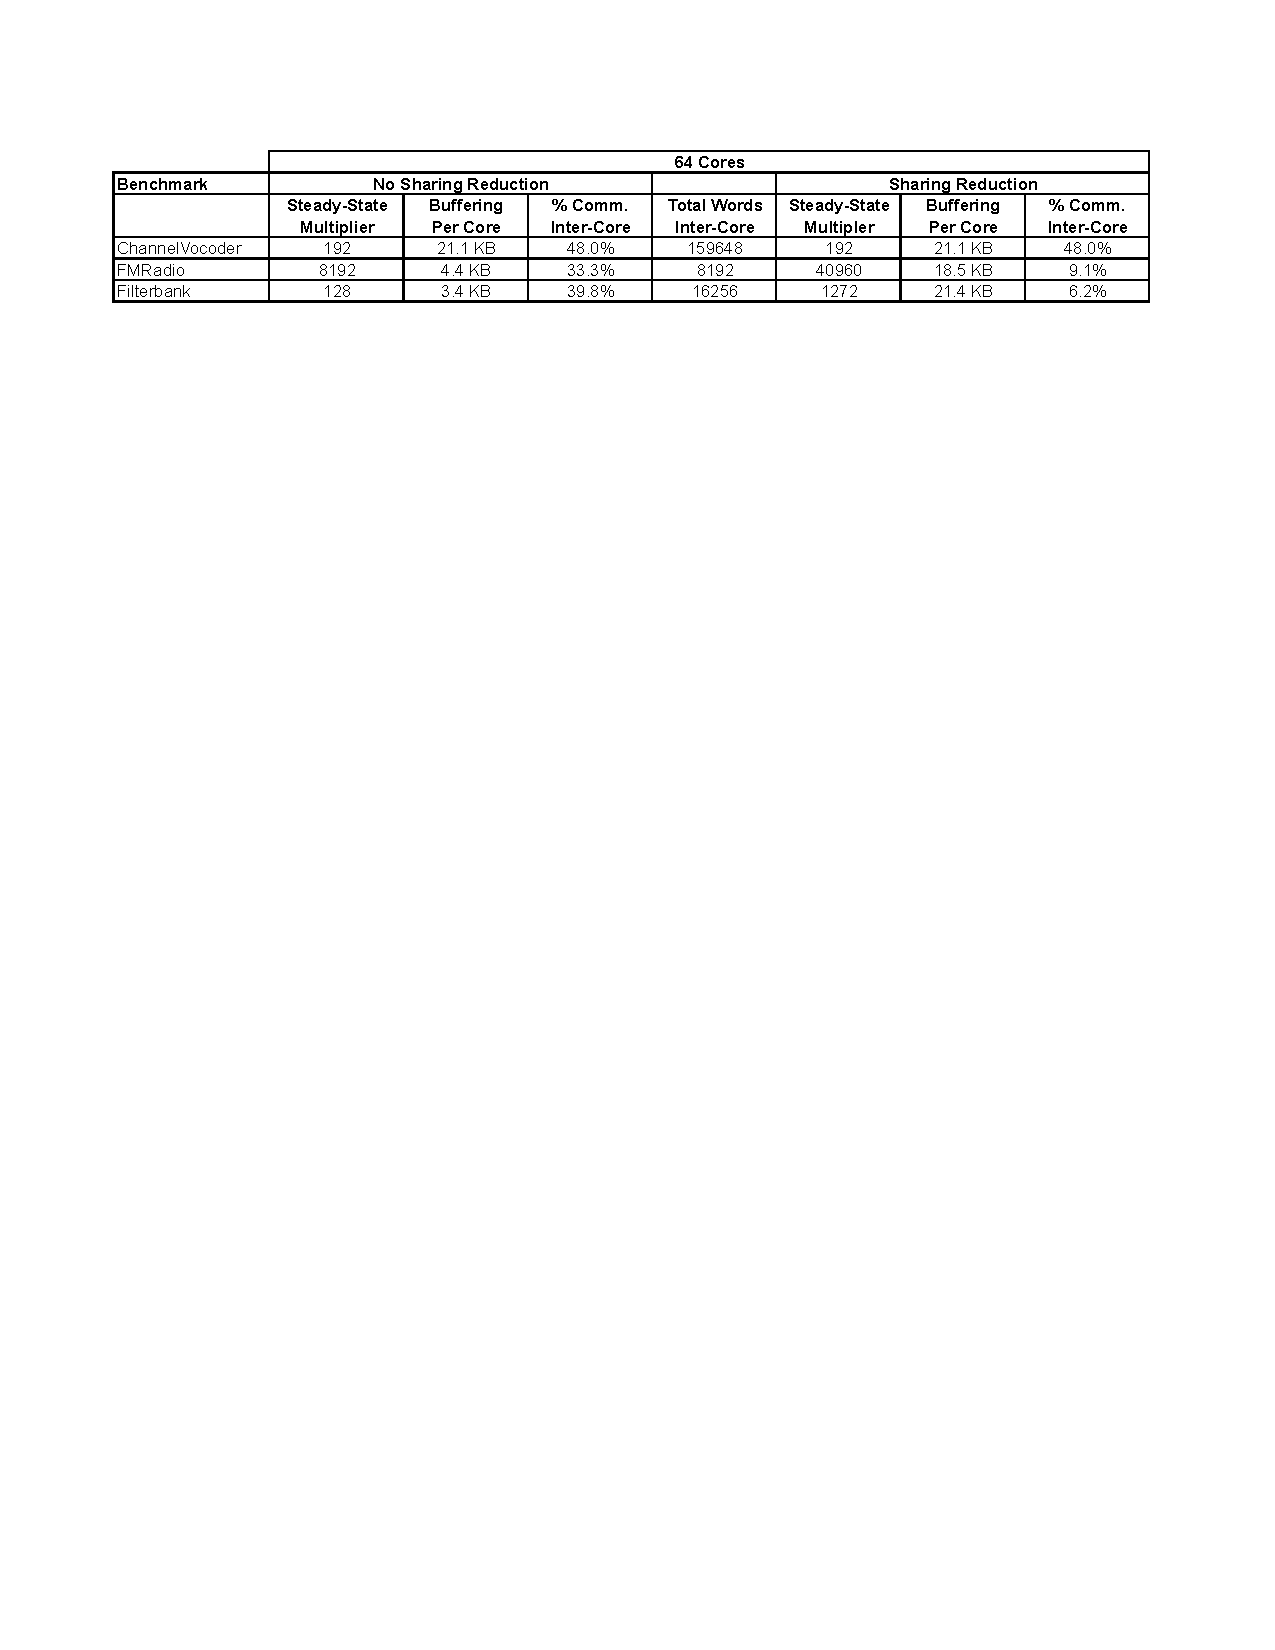
\includegraphics[width=6in]{figures/64-core-table.pdf}}
% \caption[Communication, multiplier and buffering statistics for
% benchmarks.]{
% Communication, multiplier and buffering characteristics for
% benchmarks: (a) gives the steady-state multipliers calculated for
% sharing reduction, (b) compares the steady-state with and without
% sharing reduction. 
% \label{fig:fission-table}}
% \end{figure*}

\begin{figure*}[t]
\centering
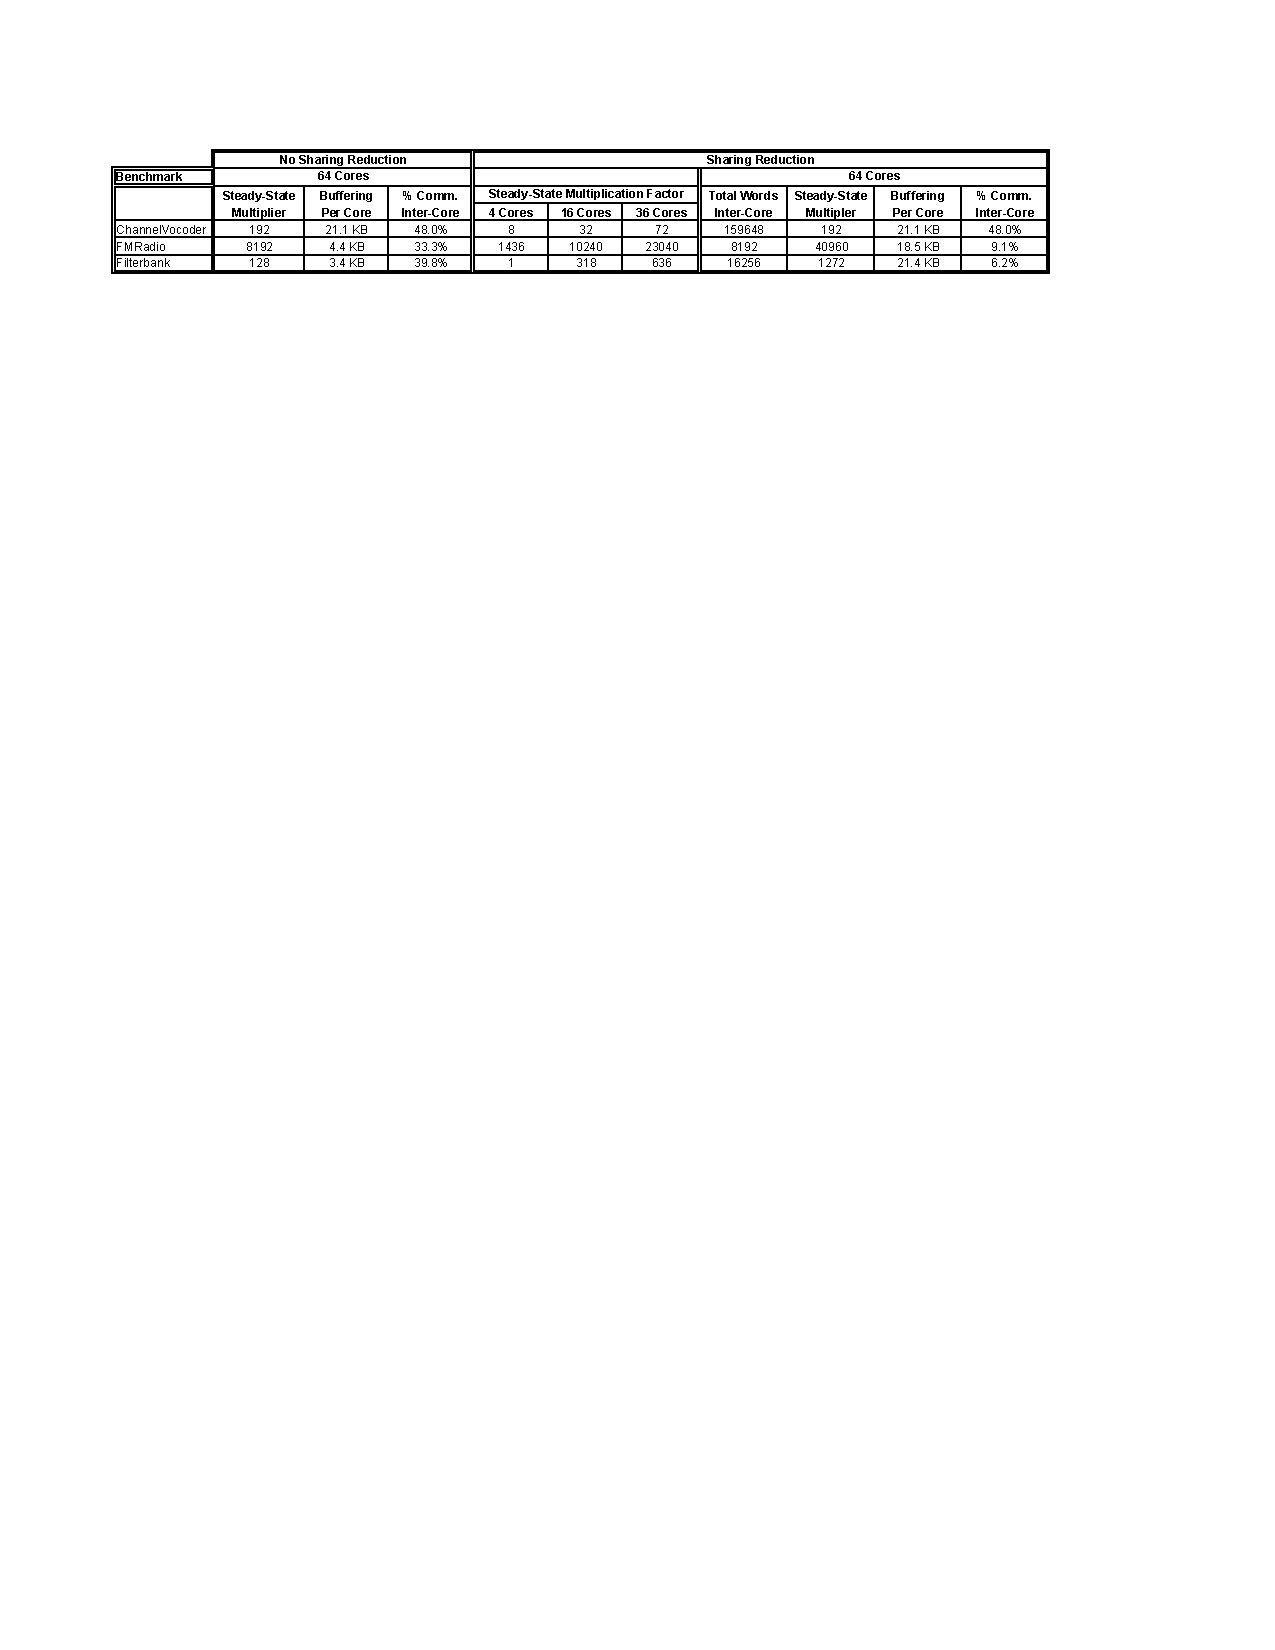
\includegraphics[width=6.1in]{figures/big-table.pdf}
\caption{\label{fig:big-table}  Steady-state multiplicity, buffering,
  and communication for fission with and without sharing reduction.}
\end{figure*}

% \begin{figure}[t]
% \centering
% 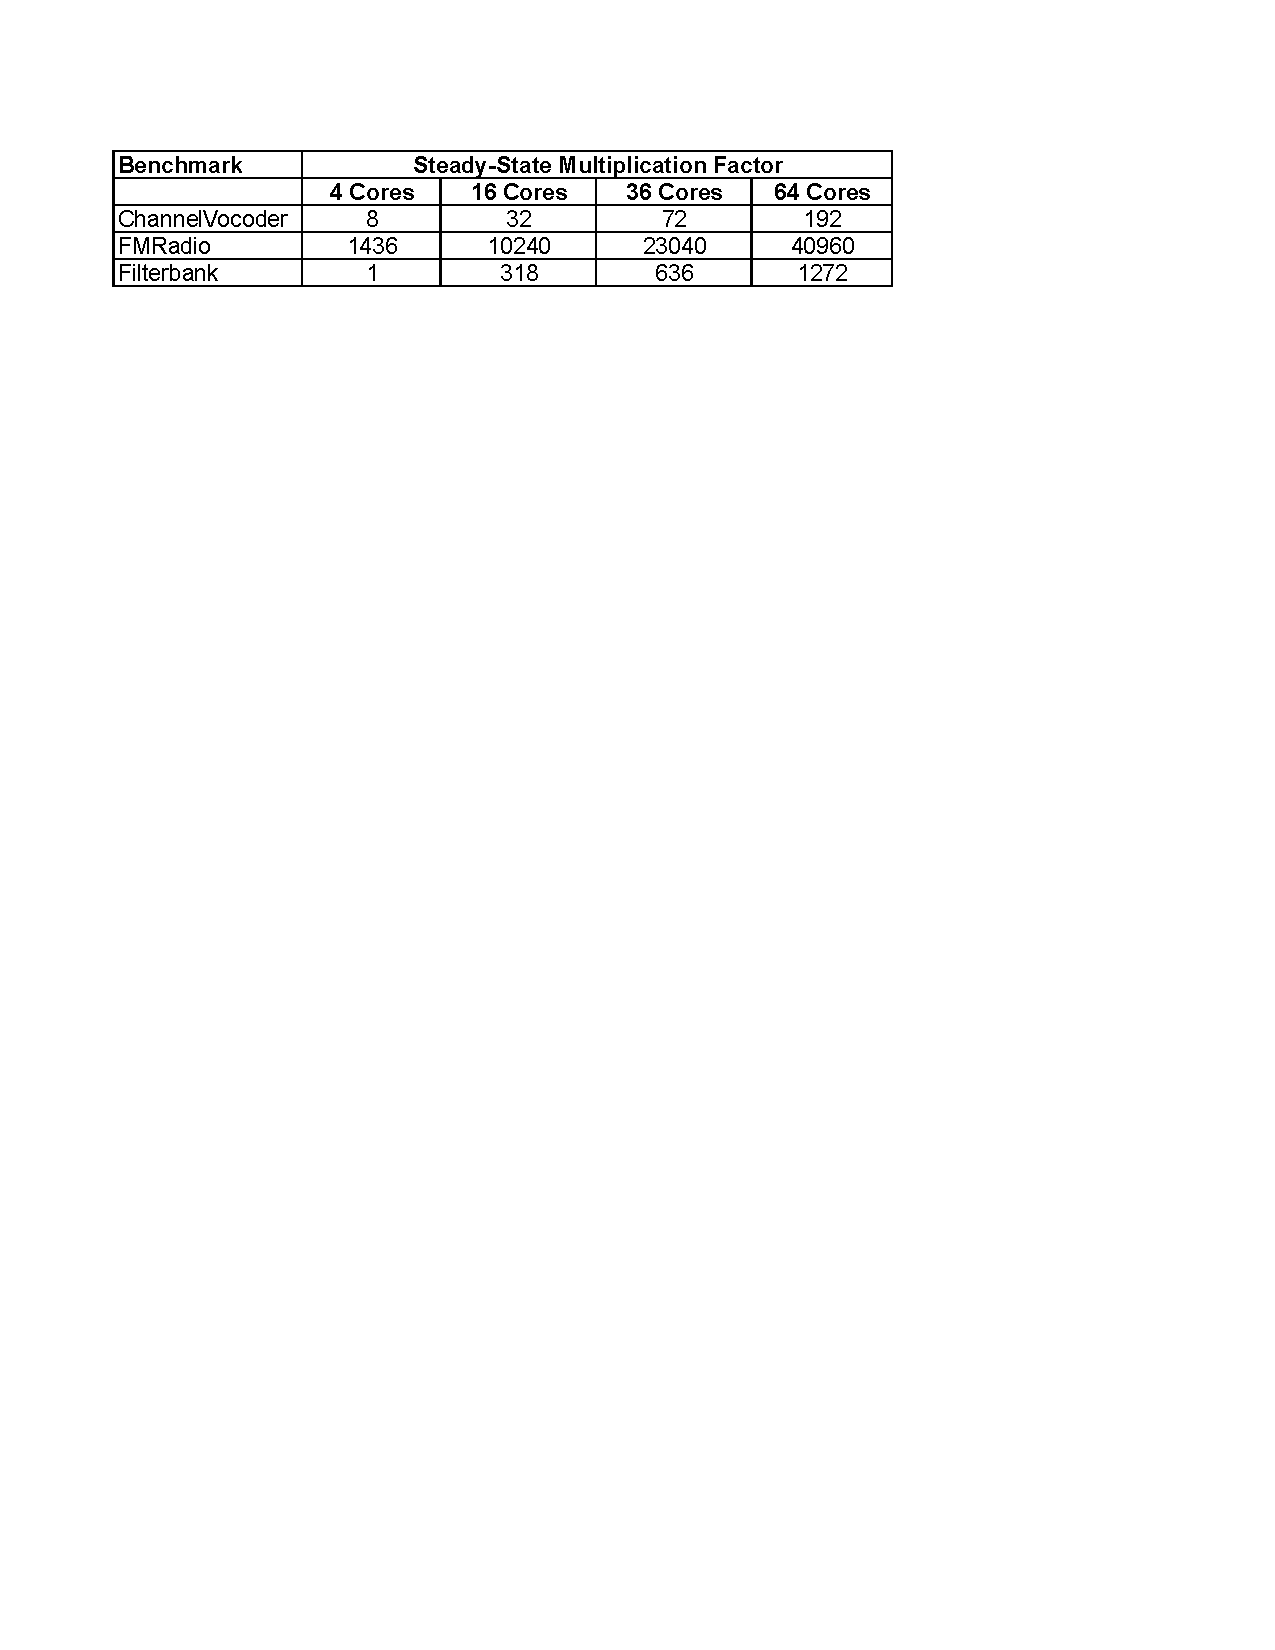
\includegraphics[width=3.3in]{figures/mult-table.pdf}
% \caption{\label{fig:mult-table}  The steady-state multipliers calculated for
% sharing reduction.}
% \end{figure}

% \begin{figure*}[t]
% \centering
% 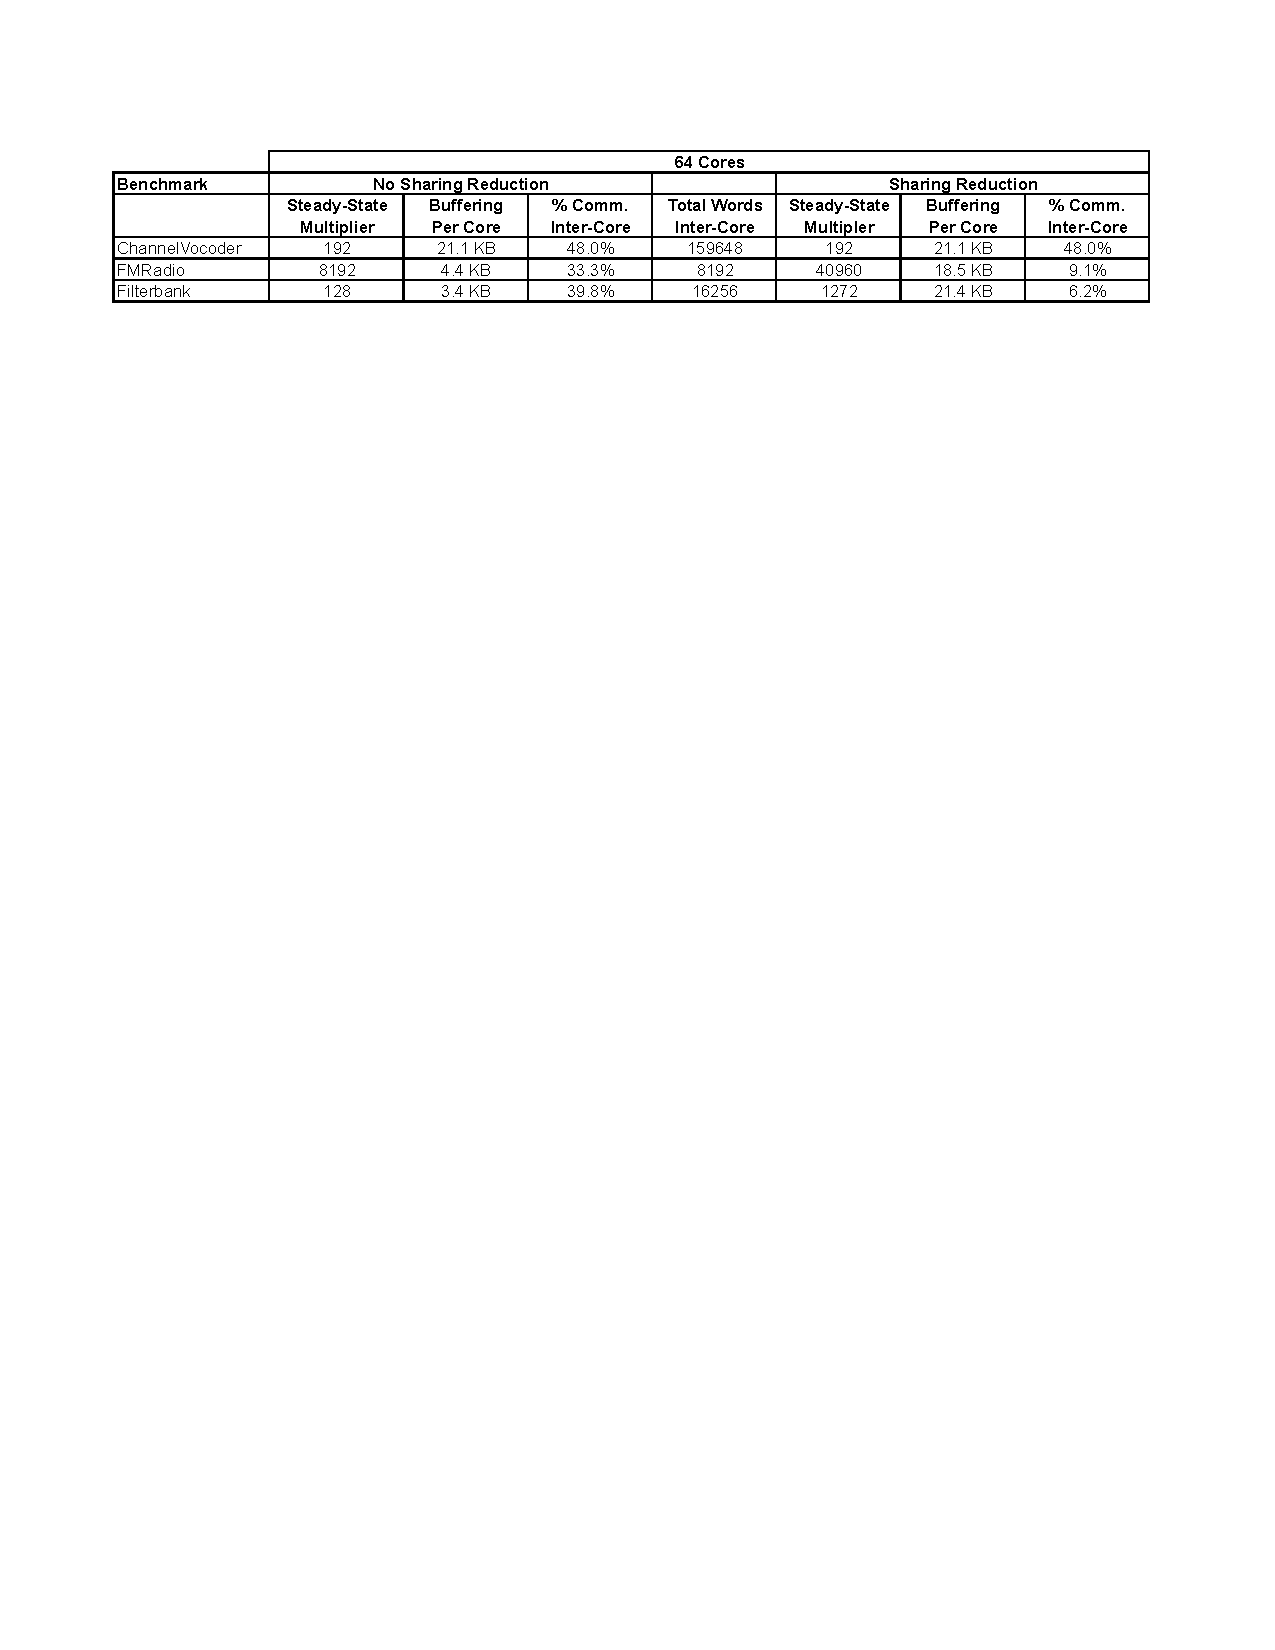
\includegraphics[width=6in]{figures/64-core-table.pdf}
% \caption{ Multiplier, buffering and communication for the steady-state with and without
% sharing reduction. 
% \label{fig:fission-table}}
% \end{figure*}

Figure~\ref{fig:big-table} compares the steady-state with and
without sharing reduction for a 64-core mapping, as well as gives the
constant $c$ calculated by sharing reduction for 4, 16, and 36.  The
factor is larger for FMRadio because one filter has $C(f) \gg o(S,
f)$.  The multiplication factor affects both latency and buffer sizes
adversely.  The application designer will have to decide if the
latency of these techniques can be borne given the application
criteria.  The total buffering requirement is increased when the
steady-state is increased.  However, since we are then fissing, the
buffer is divided amongst the fission products, and the {\it per-core}
buffering requirement is unaffected by the increase.  For example,
FMRadio, has a per-core 18 KB buffering requirement across all
configurations (4, 16, 36, and 64 cores).  This requirement fits in
the per-core L2 size of 64 KB for the Tile64.

 For ChannelVocoder,
sharing reduction has no effect because most of the peeking filters do
not satisfy $T_{\mt{apply}} = 0.05$ because of differing fission
factors between producers and consumers.  For the peeking filters that do,
the steady-state multiplier required for legal general fission for the
graph is enough to assure $T_{\mt{sharing}}$ is met.  Even though
sharing reduction has no effect for ChannelVocoder, general fission
avoids the 38\% of total items that were unnecessary duplicated by
DupDec.

For FMRadio and Filterbank, sharing reduction leads to significant
decreases in the percentage of total items communicated inter-core for
each steady-state.  The buffer requirement is increased an average of
5.2x for these benchmarks.  The total number of words communicated
inter-core during each steady-state is the same, with and without
sharing reduction.  However, the steady-state is greater in the
sharing reduction case, thus producing more outputs.

\begin{figure}[t]
\centering
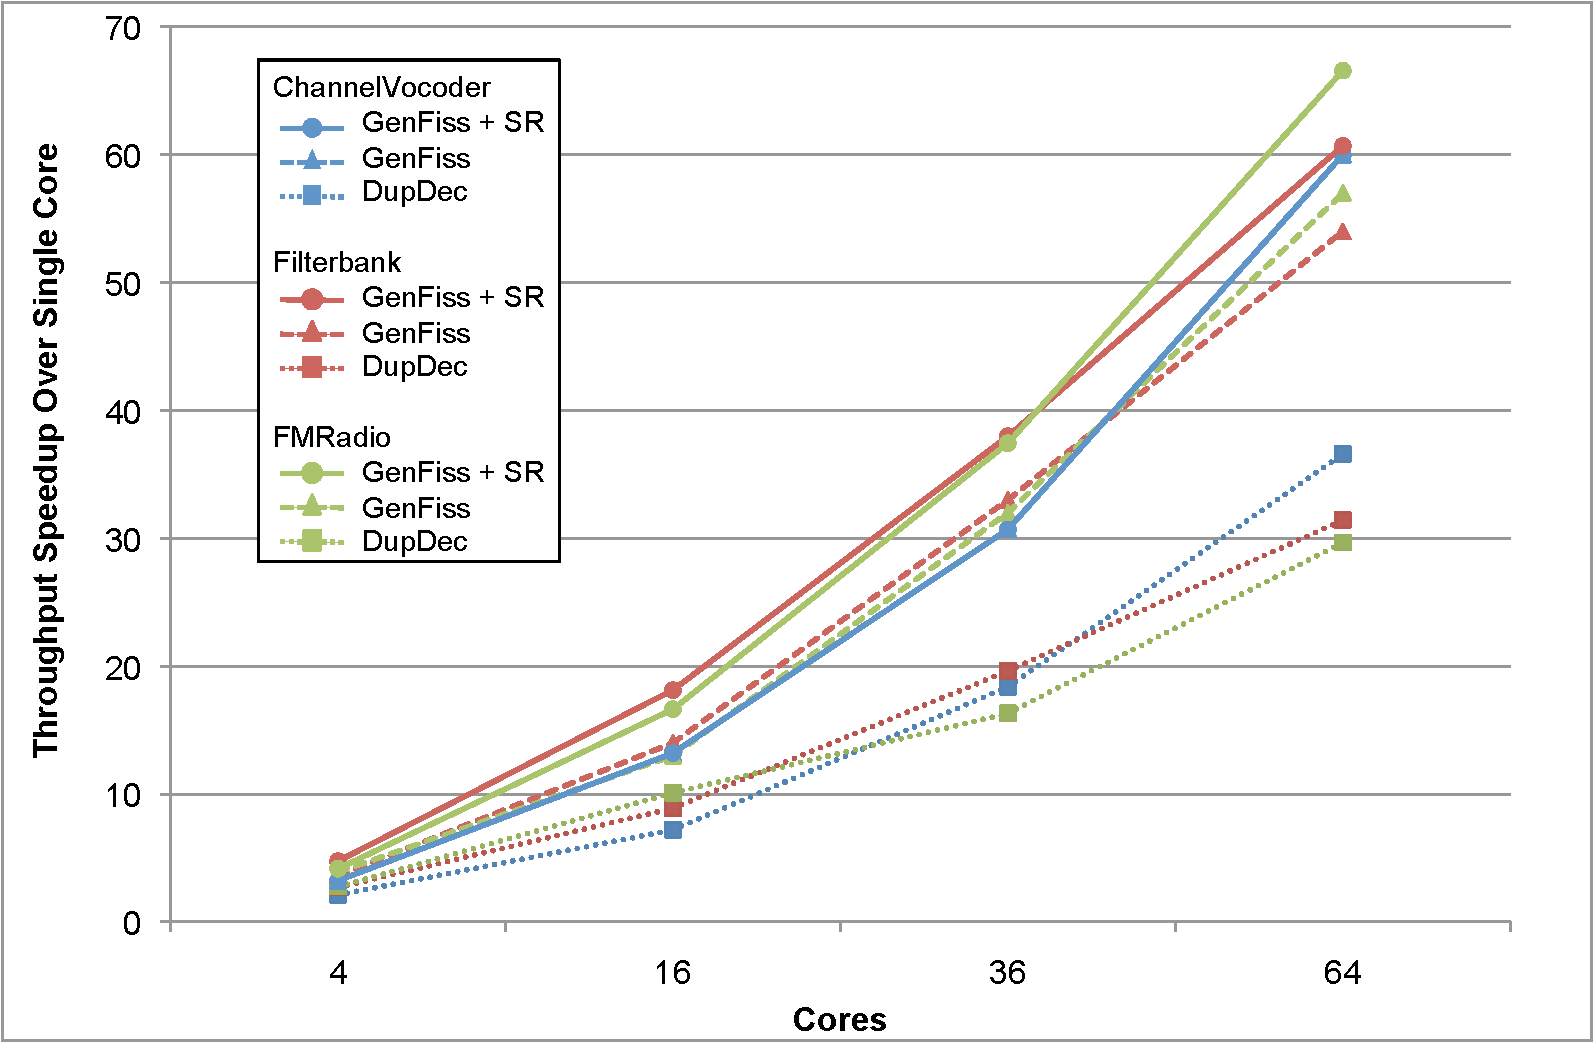
\includegraphics[width=3.3in]{figures/tilera-chart.pdf}
\caption[Comparing the fission techniques on the TILE64.]{
  Evaluation for DupDec versus general fission versus general fission with sharing reduction
  4, 16, 36, and 64 cores on the TILE64.  \label{fig:tilera-chart}}
\end{figure}

Figure~\ref{fig:tilera-chart} gives the performance results for the
Tilera TILE64 architecture.  We present results for DupDec, general
fission, and general fission with sharing reduction for 4, 16, 36, and
64 core configurations, with throughput normalized to single-core
throughput.  General fission with sharing reduction outperforms
DupDec by an average of 1.8x for the three benchmarks when targeting
64 cores. The average 64-core speedup over single core is 62.3x for the
general fission plus sharing reduction for these three benchmarks.

FMRadio experiences the most significant gain from general fission
plus sharing reduction over DupDec (67x versus 30x, respectively, for
64 cores).  FMRadio has the lowest computation to communication ratio
of the 3 benchmarks.  Furthermore, each filter of is fissed by the
number of cores targeted.  For 64 cores, each filter is fissed 64
ways.  DupDec must perform a global all-to-all communication involving
all 64 cores between each level of the graph!
 
ChannelVocoder achieves a 60x speedup for general fission over a
single core.  This is not perfectly linear because of the parallel
mapping; asymmetries exist between the extent of task parallelism and
the number of cores (see~\ref{mgordon-asplos06}).  The speedup over
DupDec (1.62x) is more modest because the width of many of the
fission applications is 3, so DupDec is duplicating input data to
groups of 3 filters.  Filterbank is similar, the width of fission is 4
for all filters when targeting 64 cores.

Sharing reduction is required to achieve scalable speedups for both
FMRadio and Filterbank.  For FMRadio, sharing reductions leads to a
17\% speedup increase for 64 cores.  This because sharing reduction
significantly reduces the number of remote write store instructions
required per output.  This affects FMRadio because of its low
computation to communication ratio.  Sharing reduction sees a 12\%
increase on Filterbank, as Filterbank has a larger computation to
communication ratio.

\begin{figure}[t]
\centering
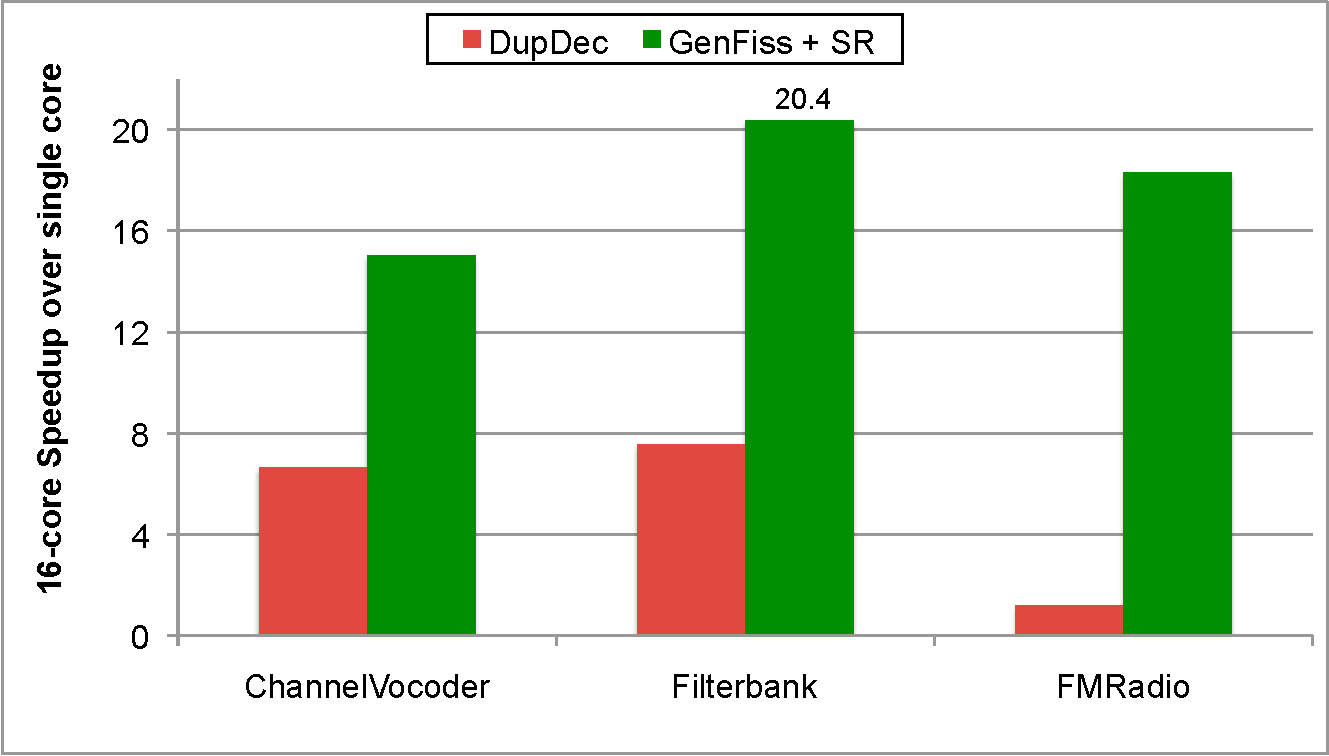
\includegraphics[width=3.3in]{figures/smp-chart.pdf}
\caption[Comparing the fission techniques on the 16-core SMP.]{
  Evaluation for DupDec versus general fission with sharing reduction
  for the 16-core SMP architecture.  \label{fig:smp-chart}}
\end{figure}

Our techniques enable scalable parallelization, with a mean speedup of
17x for our 3 benchmarks on the SMP.  Figure~\ref{fig:smp-chart} gives
the 16-core speedup comparison for DupDec versus general fission with
sharing reduction for our target SMP architecture.  The mean speedup
increase for general fission with sharing reduction over DupDec is
6.7x.  FMRadio again sees the largest speedup increase in the
comparison at 13.0x.  The reasons for this large speedup are similar
as given in the previous section.  However, the SMP communication
mechanism is not as efficient as the TILE64, thus general fission with
sharing reduction gives a greater speedup because reducing inter-core
communication has more impact.

\section{Related Work}
\label{sec:related}

% BILL

%Signal~\cite{Signal}, 
%Lucid~\cite{Lucid77}, and
%Occam~\cite{Occam}, and Sisal \cite{sisal}.
%Parallel Haskell~\cite{ph}
In addition to StreamIt, there are a number of stream-oriented
languages drawing from domains such as functional, dataflow, CSP and
synchronous programming~\cite{survey97}.  The Brook language is
architecture-independent and focusses on data
parallelism~\cite{brook04}.  Stream kernels are required to be
stateless, though there is special support for reducing streams to a
single value.  Stream\-C/Ker\-nel\-C is lower level than Brook;
kernels written in KernelC are stiched together in StreamC and mapped
to the data-parallel Imagine processor~\cite{imagine03ieee}.  SPUR
adopts a similar decomposition between ``microcode'' stream kernels
and skeleton programs to expose data parallelism~\cite{spur05samos}.
Cg exploits pipeline parallelism and data parallelism, though the
programmer must write algorithms to exactly match the two pipeline
stages of a graphics processor~\cite{cg03}.  Compared to these
languages, StreamIt places more emphasis on exposing task and pipeline
parallelism (all the languages expose data parallelim).
%and on sliding window operations (filters that peek).  
By adopting the synchronous dataflow model of execution~\cite{lee87},
StreamIt focusses on well-structured programs that can be aggressively
optimized.  The implicit infinite loop around programs is also a key
StreamIt characteristic that enables the transformations in this
paper.  Spidle is also a recent stream language that was influenced by
StreamIt~\cite{spidle03}.
%and Lucid Synchrone~\cite{Lucid-Synchrone}.
%Synchronous languages which
%target embedded applications include Esterel~\cite{Esterel},
%Lustre~\cite{Lustre}, and Additional

Liao et al. map Brook to multicore processors by leveraging the affine
partitioning model~\cite{liao06brook}.  While affine partitioning is a
powerful model for parameterized loop-based programs, in StreamIt we
simplify the problem by fully resolving the program structure at
compile time.  This allows us to schedule a single steady state using
flexible, non-affine techniques (e.g., simulated annealing) and to
repeat the found schedule for an indefinite period at runtime.
Gummaraju and Rosenblum map stream programs to a general-purpose
hyperthreaded processor~\cite{gummaraju05micro}.  Such techniques
could be integrated with our spatial partitioning to optimize per-core
performance.  Gu et al. expose data and pipeline parallelism in a
Java-like language and use a compiler analysis to efficiently extract
coarse-grained filter boundaries~\cite{du03sc}.  Ottoni et al. also
extract decoupled threads from sequential code, using hardware-based
software pipelining to distribute the resulting threads across
cores~\cite{ottoni05decoupled}.  By embedding pipeline-parallel
filters in the programming model, we focus on the mapping step.

%%%%%%%%%%%%%%%%%%%%%%%%%%%%%%%%%%%%%%%%%%%%%%%%%%%%%%%%%%%%%%%%%%%%%

Previous work in scheduling computation graphs to parallel targets has
focused on partitioning and scheduling techniques that exploit task
and pipeline parallelism~\cite{SDFSched, SDFSched2,may87communicating,
DAGSched, pipeline-sdf}.  Application of loop-conscious
transformations to coarse-grained dataflow graphs has been
investigated.  Unrolling (or ``unfolding'' in this domain) is employed
for synchronous dataflow (SDF) graphs to reduce the initiation
interval but they do not evaluate mappings to actual
architectures~\cite{unfolding,unfolding2}. Software pipelining
techniques have been applied to SDF graphs onto various embedded and
DSP targets~\cite{bakshi99,chatha-02}, but has required programmer
knowledge of both the application and the architecture. To our
knowledge, none of these systems automatically exploit the combination
of task, data, and pipeline parallelism.  Furthermore, these systems
do not provide a robust end-to-end path for application
parallelization from a high-level, portable programming language.

%% Previous work on instruction-level software pipelining has focused
%% mostly on scheduling machine instructions in a loop via modulo
%% scheduling~\cite{rau81,lam-softpipe}.  The algorithms devised must
%% account for tight resource constraints and complex instruction
%% dependences. Our software-pipelining problem is much less constrained,
%% enabling us to employ a simple greedy heuristic.  

%% Furthermore, a traditional modulo scheduling algorithm is not needed
%% because we have an implicit loop barrier at the end of each
%% steady-state.  ILP compilers for clustered VLIW
%% architectures~\cite{Bulldog,Multiflow,lee98spacetime,qian02} must
%% partition instructions and assign them to clusters as part of the
%% instruction scheduling. Clustering is analogous to our application of
%% filter fusion in our software pipelining algorithm.

%\Section{Concluding Remarks}
\vspace{-11pt}

As computer architectures change from the traditional monolithic
processors, to scalable wire-exposed and multicore processors, there
is a greater need for portable applications that expose parallelism
and communication to enable efficient and high performance
executions---while also boosting programmer productivity. StreamIt is
a programming language and a compilation infrastructure specifically
engineered to naturally expose and leverage stream abstractions that
are embodied in modern streaming applications. We have used StreamIt
to implement DSP codes (e.g., software radio, beamforming), image and
video codecs (e.g., MPEG-2 encoding and decoding), encryption
algorithms (e.g., DES and Serpent), and many other applications. The
language, compiler, and applications are available for download from
the project web page at http://cag.csail.mit.edu/streamit.

The goal of the StreamIt project is to boost productivity for
streaming application developers such that they focus on algorithmic
innovation rather than on performance tuning. The ability to leverage
domain specific language constructs affords optimization opportunities
that can deliver high performance from high levels of abstraction. 

We believe emerging languages such as X10 can provide a framework to
implement domain specific abstractions in a general purpose
programming model. We have designed and implemented a prototype bridge
to run StreamIt code as part of the X10 virtual machine. As a result,
application developers can use the streaming abstractions for the
computation that fit that model of computation, while different
abstractions can be used to describe other aspects of the computation.
A part of our ongoing work is concerned with evaluating the productivity
and performance merit of native interfaces to and from StreamIt codes.
\section{Conclusions \& Future Work}\label{ch:conc}

Streaming languages provide an excellent way to
target new multicore architectures while placing minimal
parallelization burden on the programmer. Multicore architecture such
as Cell that are designed to offer high peak performance are well
suited for streaming applications. This paper described a runtime
framework for streaming applications on multicores consisting of
\emph{i}) a common Multicore Streaming Layer (MSL) that provides
high-level primitives for schedulers, \emph{ii}) an implementation
of the MSL for an existing processor, namely Cell, \emph{iii}) a
lightweight dynamic scheduler for stream graphs, and \emph{iv}) a
static scheduler for stream graphs. The framework greatly
simplifies the task of a streaming language compiler or scheduler.

The real benefit provided by the framework, in particular the MSL
runtime library, is that it allows a scheduler to think directly in
terms of filters and how they are scheduled instead of lower-level
architecture-specific details. It requires far less code to implement
scheduling patterns on top of the library than directly on Cell
hardware for example, and the MSL library also allows far more complex
patterns to be implemented than directly at a lower level.
 The library running the data-parallel
fused FFT benchmark produces a reasonably small amount of overhead
(1.2\%), and the dynamic scheduler running the pipelined version of
the benchmark produces an acceptable amount of overhead (8.6\%).

The MSL library currently provides two orthogonal branches that can be
further developed. First, it is important to reduce the 9\% overhead
observed in the pipelined FFT tests involving the dynamic
scheduler. This overhead is entirely due to the cost of the run list
when many commands are active, and it can probably be significantly
reduced by optimizing library code, although it is also likely that
doing so would make the SPE library implementation, especially the run
list, much more specialized.

In addition, the implementation currently lacks real support for
filters with dynamic rates (i.e. I/O rates that change over time and
across executions)
-- the library simply leaves the
responsibility of tracking rates to the scheduler entirely. Feedback
from the library on how much data filters have produced and consumed
would be very useful for schedulers; ultimately, the library should
have some way of running filters with unbounded dynamic rates. The
latter would require a general mechanism to suspend dynamic rate
filters in the middle of executing their work functions.

The dynamic scheduler can be extended in many directions. The simplest
additions involve adjusting the metric used for selecting filters to
test and improve the performance of the dynamic scheduler as work
becomes more and more imbalanced between filters. In addition, an
important advantage of dynamic scheduling in general is the ability to
react to dynamic rate filters and the runtime distribution of work in
the stream graph; implementing robust support for dynamic rate filters
in the stream graph would drastically increase its usefulness.


%\section{Acknowledgements}

We are very grateful to Anant Agarwal, Mike Taylor, Davind Wentzlaff,
Walter Lee, Matt Frank, and the rest of the Raw group for their
development of the Raw infrastructure and wholeharted support of this
project.  This work is supported in part by a grant from DARPA (PCA
F29601-04-2-0166), an award from NSF (CISE EIA-0071841), and a
fellowship from the Singapore-MIT Alliance.

\enlargethispage{\baselineskip}
\setlength{\bibspacing}{0pt}
\begin{scriptsize}
\bibliographystyle{abbrv}
\bibliography{references}
\end{scriptsize}

\end{document}
